

\chapter{Diffraction in a perfect crystal} % Main chapter title
\label{Chap:Diffraction} 


In the previous chapter we have dusted off the tool-kit required to tackle diffraction. The current chapter deals with the theoretical formalism of electron diffraction and shows the explicit path of applying this formalism to group-III nitride compounds. 


Since I believe some insight into the theory comes from the chronological development of the current accepted models, I'll treat my reader to the historical background of diffraction on page~\pageref{sec:history}. Historically, diffraction is associated with X-rays, and we will end up using parts of the theories developed for X-ray diffraction when talking about electron diffraction. 

While the phenomenon is described by the same physics regardless of the type of particles used, the way individual diffracting particles interact with matter can differ. While X-rays diffract from the electron density in the crystal, electrons are scattered elastically by the Coulomb potential. The latter is related to the electron density via the Poisson equation and, additionally, it also includes the nuclear contributions. Similarly, neutrons interact mainly with the nuclear potentials in the crystal sample. Table~\ref{table:diffractingParticles} shows the properties of the most common types of particles used in diffraction experiments together with their scattering sources.

\begin{table}[!h]
\caption{Particles used in diffraction experiments together with their scattering properties.}
\label{table:diffractingParticles}
\centering
\begin{tabular}{ l l c l}
\toprule
\tabhead{Particle} & \tabhead{$\lambda$ [nm]} &\tabhead{Charged?} &\tabhead{Scattering object}\\
\midrule
  X-ray photon \hspace{0.2cm} & $ 0.01 - 1.0$    & no   & electron density distribution\\
  neutron                     & $\sim 0.1$    & no   & atomic nuclei distribution\\
  electron                    & $0.001 - 0.1$  & yes  & atomic potential distribution  \\
\bottomrule
\end{tabular}
\end{table}

Compared to X-rays, electrons have significantly shorter wavelengths and are scattered much more strongly by matter. This means that electrons convey information about much smaller crystal volumes than conventional X-ray microscopy, in other words, they promise better spatial resolution. It also means that effects which are negligible when it comes to the  interaction of X-rays with matter, cannot be swept under the carpet and ignored when it comes to electrons. While we can  use the geometrical, \ie kinematical, model for predicting X-ray diffraction intensities,  we need to take into account the fact that electrons   will lose energy and coherence on their paths through the sample and that electron waves are more strongly coupled to each other. To do this we must turn to the dynamical theory for the prediction of scattered electrons intensities. More on that on page~\pageref{sec:kinvsDyn}.

I have already made the note that diffraction is chiefly related to the wave behaviour of small particles like photons, electrons or neutrons. This behaviour is mathematically written in the form of a Bloch wave $\psi(\mathbf{r})$ whose squared amplitude, $|\psi(\mathbf{r})|^2$, describes the probability density of finding the particle at position $\mathbf{r}$. We will see on page~\pageref{sec:DHW} that these wavefunctions satisfy the Schr{\"o}dinger's equation inside a crystal described by a periodic potential $V_C(\mathbf{r})$. Finding this crystal potential is the journey we will explore in the first part of this section.

In layman terms, diffraction is the phenomena of directional scattering arising as constructive interference along certain directions and destructive interference along others. From the intensity of the interfering waves one can derive information on the spatial distribution of the scattering centres and we will see how that relates to directional elastic scattering. We will talk chiefly about the crystal planes which dictate the Bragg scattering direction.
I will also talk about the interaction of the electrons with the unit cell, which affects the intensity of the diffracting beam along chosen direction through the parameter known as the \textit{scattering factor}. There are always these two conditions to take into account when figuring out the diffraction intensity along a certain direction. And both of these parameters (scattering angle from lattice plane and scattering factor) can have values for which the diffraction beam intensity vanishes. Which is why we divide the following sections into \textit{Diffraction geometry} on page~\pageref{sec:geometry} and  \textit{Diffraction intensity} on page~\pageref{sec:intensity}.





We will be covering some of the theoretical aspects of diffraction in this section. For a thorough and in-depth description of diffraction and it's application in crystallography we suggest the reader find a copy of the \emph{International Tables of Crystallography Volume B: Reciprocal space}~\cite{IntTableCrysBX, IntTableCrysBe}. 


%%%%%%%%%%%%%%%%
\section{Short historical overview}
\label{sec:history}
Soon after systematically experimenting with generating what will end up being known in the English languages as \textit{X-rays}, the German physicist Wilhelm R{\"o}ntgen used this new form of high energy radiation to ``take a picture'' of his wife’s hand. To everyone’s amazement the picture taken in 1895 showed the bones of her hand wearing her wedding ring. While the medical applications of X-rays are impressive in their own right, a material scientist will claim that the best application of X-rays was yet to come.

Not even twenty years later, another German physicist, Max von Laue, decided to use this new radiation, which he'd probably called R{\"o}ntgen rays,  to ``take a picture'' of a crystal. He actually had a good reason to try that. Von Laue expected the wavelength of these radiations to be of the same order of magnitude as the distance between atoms in matter. If this criterion is met then the wave behaviour of the radiation will suffer constructive interference along directions dictated by the crystal lattice planes. What he observed in his image was a series of ordered spots which would end up telling a story about the particular ordered arrangement of the crystal atoms. From here on things move rather quickly. Table~\ref{table:historyDiff} shows a quick overview over about a hundred years of historical events building to the development of electron diffraction techniques.

It is interesting to notice the interplay between experimental observations and theoretical predictions in the development of diffraction as a field. The observation of X-ray diffraction supported, first of all, the controversial wave-like behaviour of particles narrative, and, second of all, the description of crystalline materials as periodic lattice structures. It also led to the development of Bragg's law. Moreover, since the theory of space group symmetry had already been developed by the Russian crystallographer E. S. Fedorov, X-ray diffraction quickly became the structure analysis tool of choice of crystallography.








  

\renewcommand{\arraystretch}{1.3}

\begin{table}[htpb]
\caption{Partial chronology of the history of diffraction. }
\label{table:historyDiff}
\centering
\begin{tabular}{p{1.2cm}p{11cm}}
\toprule
\tabhead{Year} & \tabhead{Event} \\
\midrule

  {\small 1912} & {\small First X-ray diffraction experiments by W. Friedrich, P. Knipping and M.~von Laue( i.}  \\
  
  {\small 1913} & {\small Bragg family derives their name bearing law~\cite{Bragg13} to describe the geometry of diffraction spots.}\\
  
  {\small 1914} & {\small C. G. Darwin~\cite{Darwin14} derives the first dynamical theory for the intensities of the diffraction spots.}\\
   
  {\small 1924} & {\small L. de Broglie hypothesises that particles should also behave as waves.}\\
  
  {\small 1927} & {\small Independently, G. P. Thomson~\cite{Thomson27} at the University of Aberdeen and C. J. Davisson and L. H Germer~\cite{Davisson27} at the Bell Labs, observe low energy electron diffraction spots through thin films.}\\
     
  {\small 1928} & {\small H. Bethe~\cite{Bethe28} uses eigenvalue equations to explain and predict intensities in electron diffraction images.}\\
      
  {\small 1928} & {\small First electron diffraction patterns are recorded by S. Nishikawa and S.~Kikuchi~\cite{Nishikawa28} from grazing incidence geometry and are described as ``black and white lines in pairs due to multiple scattering and selective reflection''.}\\

  {\small 1931-4} & {\small E. Ruska and M. Knoll build the first electron microscope (EM), later known as a direct or transmission EM (TEM). }\\
  
  {\small 1935-8} & {\small M. Knoll suggests the idea of a scanning EM (SEM). M. von Ardenne~\cite{Ardenne38} constructs the first one.}\\
  
  {\small 1961} & {\small A. Howie and M. J. Whelan~\cite{Howie61} expands Darwin's theory to develop a simultaneous differential equation form for electron diffraction applicable for predicting diffraction contrast.}\\
  
  {\small 1960-5} & {\small P. B. Hirsch and co-workers at Cambridge~\cite{Hirsch60, electronMicroscopy} develop the theory of electron diffraction contrast which can be used to identify line and planar defects in thin films in TEM images.}\\
 
  {\small 1967} & {\small D. G. Coates~\cite{Coates67} observes electron diffraction patterns in the SEM later labelled electron channelling patterns (\textbf{ECPs}). }\\
  
  {\small 1967} & {\small  G. R.~Booker~\cite{Booker67} provides a theoretical interpretation for the phenomena based on the Darwin-Howie-Whelan theory. He also notices that the backscattered intensity varies rapidly with orientation close to Bragg condition, which will develop in a new technique of its own known as electron channelling contrast imaging (\textbf{ECCI}).}\\

    {\small 1973} & {\small J. A. Venables and C. J. Harland~\cite{Venables73} describe another diffraction technique capable of providing local crystallographic information termed electron backscattering patterns (\textbf{EBSP}) or latter electron backscattered diffraction (\textbf{EBSD}). }\\
  
   {\small 2012} & {\small The latest diffraction technique in the SEM with improved spatial resolution compared to EBSD is reported as transmission EBSD (\textbf{t-EBSD}) by R. R. Keller and R. H. Geiss~\cite{Keller12} and Transmission Kikuchi Diffraction (\textbf{TKD}) by P. W. Trimby~\cite{Trimby12}. }\\
\bottomrule
\end{tabular}
\end{table}
\renewcommand{\arraystretch}{1.}

While Bragg's law was good enough to explain the geometry of the diffraction spots, it proved inconsistent in predicting experimental X-ray diffraction intensities. This lead C. G. Darwin to develop a first form of dynamical diffraction theory. He took into account the interaction of X-rays with matter as partially transmitted and partially reflected amplitudes at each lattice plane. His theory predicted correct values for the reflected intensities. Later, in 1917, P. P. Ewald introduced a new form of dynamical theory in which he considered the crystal to be a periodic distribution of dipoles excited by the incident wave. The new theory predicted both transmitted and reflected intensities. 

There were still limitations in the dynamical theories. In 1930, J. A. Prins~\cite{Prins30} modified Darwin's theory to take into account the fact that the crystal is an absorbing medium. Just a year later, in 1931, von Laue showed that the interaction in Ewald's theory can be described by solving Maxwell's equations in a continuous medium with dielectric susceptibility distributed periodically in three dimensions. It is in this form that the dynamical diffraction theory is most used today and also the one we will use in this work.
  
The inverse effect was triggered by de Broglie's doctoral thesis in which he speculates that all particles ought to also behave as waves. The discovery of the remarkable phenomena that is electron diffraction provided the experimental means for the development of quantum mechanics. It soon became apparent that the diffraction theory must again be expanded to account for the more complex electron interaction with matter. Indeed, a number of dynamical theories for electrons have been developed over the years all carrying the legacy of X-ray diffraction theoretical interpretations.   

Electrons diffracting through crystals gives access to a plethora of information. When, in 1928, Shoji Nishikawa and Seishi Kikuchi directed a beam of \SI{50}{\kilo \electronvolt} electrons on a calcite sample at a grazing incidence of \SI{6}{\degree} diffraction was a phenomena associated with spots. But they have seen ``... black and white lines in pairs due to multiple scattering and selective reflection'' which we now recognise as diffraction patterns. A number of studies quickly followed the investigation of this new band features in electron diffraction. Notable here is that in 1937 Boersch~\cite{Boersch37}(paper in German) already proposed that these observations could be explain using von Laue's dynamical theory of electron diffraction.


In 1948, a number of models have already been proposed to explain the full range of features in the Kikuchi patterns. Artmann~\cite{Artmann48} (paper in German) used the reciprocity law and solved the Schr{\"o}dinger equation for bound electrons in the three dimensional crystal potential to predict with good accuracy the intensity profile and geometry of Kikuchi bands. 

While a beautiful physics experiment, electron diffraction would have lacked practical application before the development of the electron microscope; first the direct mode in 1934, where electrons penetrated through a sample and the image was collected on the other side (TEM) and, a few years later, the scanning mode, in which the incident electron beam scans over the sample in a raster manner and the backscattered electrons are recorded one ``pixel'' at a time to form an image (SEM). 

More insights could be derived from the electron signal. The diffraction spots observed in the TEM or when at a grazing incidence angle in the SEM (both conditions in which the crystal volume with which the electron beam interacts is small enough to approximate the behaviour to kinematical diffraction) were identified to be related to the crystal structure. The electron channelling patterns (ECP) observed now in the SEM can provide  information on the bulk crystal structure and orientation. If the detector is placed in the SEM such that mostly forward scattered electrons are collected, then one can obtained Kikuchi lines (EBSD) from a very small crystal volume or, in the language of microscopy, high spatial resolution.


The timely development of models and computer-aided indexing solutions for patterns from all seven crystal systems meant that fully automated EBSD could replace X-ray pole figure measurements for texture analysis avoiding the limitation that come with X-ray analysis where the sample is tilted through large angles. The model developed by Howie and Whelan for electron diffraction intensity predictions in the TEM could be easily be modified and implemented on a computer, as Hirsch had shown, to account for dislocations displacement fields and therefore predict dislocation contrast in transmission mode open the world of defect characterisation. 


Even for far from perfect crystals, electron diffraction can provide great insight. By scanning over a micro-granular crystal in the SEM and recording the EBSD image for each pixel, one can pick up the orientation of individual grains using orientation indexing techniques. In the world of material science this is extremely powerful as a tool for mapping the quality of a new material in terms of its grains.  We will talk more in Chapter~\ref{chap:TKD} about the novel Kikuchi diffraction technique, known as TKD, that can increase the spatial resolution even further allowing the study of truly nano-structural materials.

By the late 80s and early 90s, with the development of computers,  we start talking about  pattern indexing software systems. A number of companies have focused on developing modern EBSD systems packaged with indexing software appeared and experienced reasonable success catering to the industry's requirements. Unfortunately, it also marked the steady decline of academic interest in open electron diffraction software. In chapter~\ref{chap:TKD} I describe one such unicorn, and how the TKD modality was implemented and what the models are predicting. 


In about the same time when EBSD was becoming popular in the world of material science, a new SEM diffraction technique was also gaining traction. If the geometry was such that the incident beam was close to a Bragg condition, high contrast around small crystallographic defects could be observed in the recorded images, similar to the case in TEM. This technique which will be known as electron channelling contrast imaging (ECCI). Since Booker already hinted at theoretical interpretation of these effects in relationship with the available Darwin-Howie-Whelan model, the next obvious step is  to extend and implement the dynamical model such that it takes into account such small phase perturbations and can predict contrast profiles for dislocations observed in SEM. This is exactly what I endeavour to do in  Chapter~\ref{chap:ECCI}. 




%%%%%%%
\section{Kinematical versus dynamical theory}
\label{sec:kinvsDyn}
The geometrical or kinematical diffraction theory, developed for X-rays, assumes that each incident wave is scattered only once in the sample and all other interactions can be ignored. This, in turn, implies that  1) the amplitude incident on each of the diffraction centres is the same and 2) the sum of the diffracted amplitude is the sum of individual amplitudes diffracted by each diffraction centre. Therefore, the geometrical phase difference between diffracted beams is the main contributor to the diffraction pattern and the distribution of diffracted amplitudes in reciprocal space is the Fourier Transform of diffraction centres in real space.  

The integrated elastically scattered intensities predicted by the kinematical theory are proportional to the square of the structure factor and also with the crystal volume with which the incident wave interacts. Because no loss of amplitude is taken into account, the kinematical theory predicts that as the interaction crystal volume increases to infinity so would the intensity of the diffracted beam. This is obviously nonsensical for anything but very small crystals. We can conclude that the kinematical approach holds well only for relatively weak interactions (X-ray interaction with matter) and/or small crystals. Darwin~\cite{Darwin22} extended this theory and showed it can also be applied to large but defected crystals. Additionally, there is no phase information tracked in the kinematical theory and this becomes important for multiple reflections. 
 
\renewcommand{\arraystretch}{1.1}
\begin{table}[!htbp]
\caption{Kinematical vs. dynamical diffraction theories. }
\label{table:kinVsDyn}
\centering
\begin{tabular}{l | l}
\toprule
\tabhead{Kinematical theory} & \tabhead{Dynamical theory} \\
\midrule
weak interaction                           & strong interaction \\
small crystal OR large defected crystal    & infinite crystal \\
single scattering                          & multiple scattering ``pendell\"{o}sung''\\
assumes no loss                            & takes loss into account\\
no phase information                       & carries information about phase\\
intensity $\propto |F_{hkl}|^2$            & intensity $\propto |\psi_g|^2$\\
\bottomrule
\end{tabular}
\end{table}
\renewcommand{\arraystretch}{1.}

Electrons manifest wave properties similar to those of X-rays and their diffraction behaviour in crystals is in many ways analogous to that of X-rays. Nevertheless, it should be obvious by now to the careful reader that the single scattering approximation of the kinematical theory will not be suitable for the strong interactions of electrons in crystals composed of more than a few layers.  For these reasons the dynamical diffraction theory for fast electrons has been developed and applied to quantitatively interpret electron diffraction patterns. 




\section{Diffraction geometry}
\label{sec:geometry}
Having set the context of diffraction as a means of identifying the crystal structures of elements and compounds, we will now explore further the governing rule of the phenomena, that of the Bragg's law. On page~\pageref{Sec:Bragg} I reminded the reader of the geometrical conditions for constructive interference to occur. The condition was given in terms of real space parameters which is why this form is also known as the real space Bragg's condition.

But we can translate the diffracted beam in  Fig.~\ref{Fig:Bragg} such that it has the same origin as the incident beam as shown in Fig.~\ref{Fig:Ewald}. Here we label the incident beam wave vector by $\mathbf{k_0}$ and the diffracted beam wave vector by $\mathbf{k_g}$. Their origin is denoted by $C$. From the definition of elastic scattering processes, we know that the length of wave vectors $\mathbf{k_0}$ and $\mathbf{k_g}$ must be the same: $|\mathbf{k_0}|=|\mathbf{k_g}| = 1/\lambda$. It is interesting to write out the distance $OG$ between the endpoints of these vectors:

\begin{equation*}
OG = |\mathbf{k_0}|\sin{\theta_B} + |\mathbf{k_0}|\sin{\theta_B} =\frac{2\sin{\theta_B}}{\lambda}=\frac{1}{d_{hkl}}=|\mathbf{g}_{hkl}|.
\end{equation*}
where we made use of Bragg's law in the penultimate equality.




%%%%
\subsection{Bragg's law in reciprocal space -- Ewald sphere}
\label{sec:Ewald}
Now that we have reviewed  all the relevant physical names we can rewrite the Bragg's law in terms of parameters defined in the reciprocal space:
\begin{equation}
\label{eq:Bragg1}
    \mathbf{k_g}=\mathbf{k_0}+\mathbf{g}.
\end{equation}

With this equality Ewald showed that we can rephrase Bragg's equation to say: \textit{If we consider a sphere of radius $|\mathbf{k_0}|=1/\lambda$ centred at the origin of the incident beam vector, then a plane \hkl(hkl) will diffract the beam if the reciprocal lattice point $\mathbf{g}_{hkl}$ lies on that sphere.} This reciprocal space geometrical construction is known as the \textit{Ewald sphere}.  Even though we will relax this diffraction condition very soon, the Ewald sphere remains a core tool when talking about diffraction. 

 \begin{figure}
    \centering
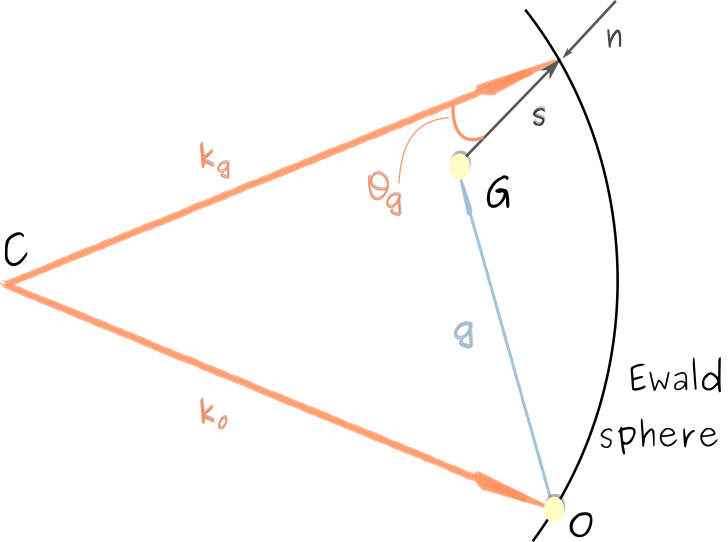
\includegraphics[width=0.52\linewidth]{Figures/EwaldSphere.png}
\caption{Ewald sphere construction in the exact Bragg condition. }
\label{Fig:Ewald}
\end{figure}
%---------

For instance, when we rotate or tilt the sample with respect to the incident beam until we hit a diffraction condition, we move the incident beam wave vector with respect to the lattice, and with it the Ewald sphere, until  a reciprocal space lattice points lies on the the sphere. Note that this is a 3D construction and we only show in the figure above a 2D projection of it.

The lengths in Fig.~\ref{Fig:Ewald} are also grossly exaggerated. For high energy electrons the wave vectors are long with respect to a much denser lattice than shown here. Drawn to scale, the portion of the Ewald sphere showing first order diffraction will be almost flat and the likelihood of multiple lattice points lying on the sphere would be somewhat increased.   



 Knowing all its parameters we can also write out the equation of the Ewald sphere. If we set the origin, $O$, to be to be the endpoint of the incident beam wave vector, then the centre of the sphere is at position $-\mathbf{k}$. For any reciprocal lattice vector $\mathbf{q}$, we can tell if it lies on the Ewald sphere if the following is true:
 \begin{equation*}
     \mathbf{q} \cdot (2 \mathbf{k}_0 + \mathbf{q})=0.
 \end{equation*}
When we enforce $\mathbf{g}$ to be on the Ewald sphere and use Eq.~\ref{eq:Bragg1}, the above becomes:
\begin{equation}
    \label{Eq:recBragg}
    \mathbf{g}\cdot (2 \mathbf{k}_0 + \mathbf{g})=\mathbf{g} \cdot (\mathbf{k}_0 + \mathbf{k}_g)=0.
\end{equation}
 This is known as the Bragg equation in reciprocal space and it tells us that the vector $\mathbf{k}_0 + \mathbf{k}_g$ must be on the plane normal to  $\mathbf{g}$ for the exact Bragg condition to be met (see Chapter 2 in  ref.~\cite{MarcTEM03} for more details). 
 




 




As useful as the reciprocal space description of the diffraction condition is, we need to introduce a real space parameter which will prove essential: the normal to crystal sample surface.

%
\subsection{Diffraction geometries}
\label{sec:diffracGeom}
%---------
\begin{figure}[ht]
    \centering
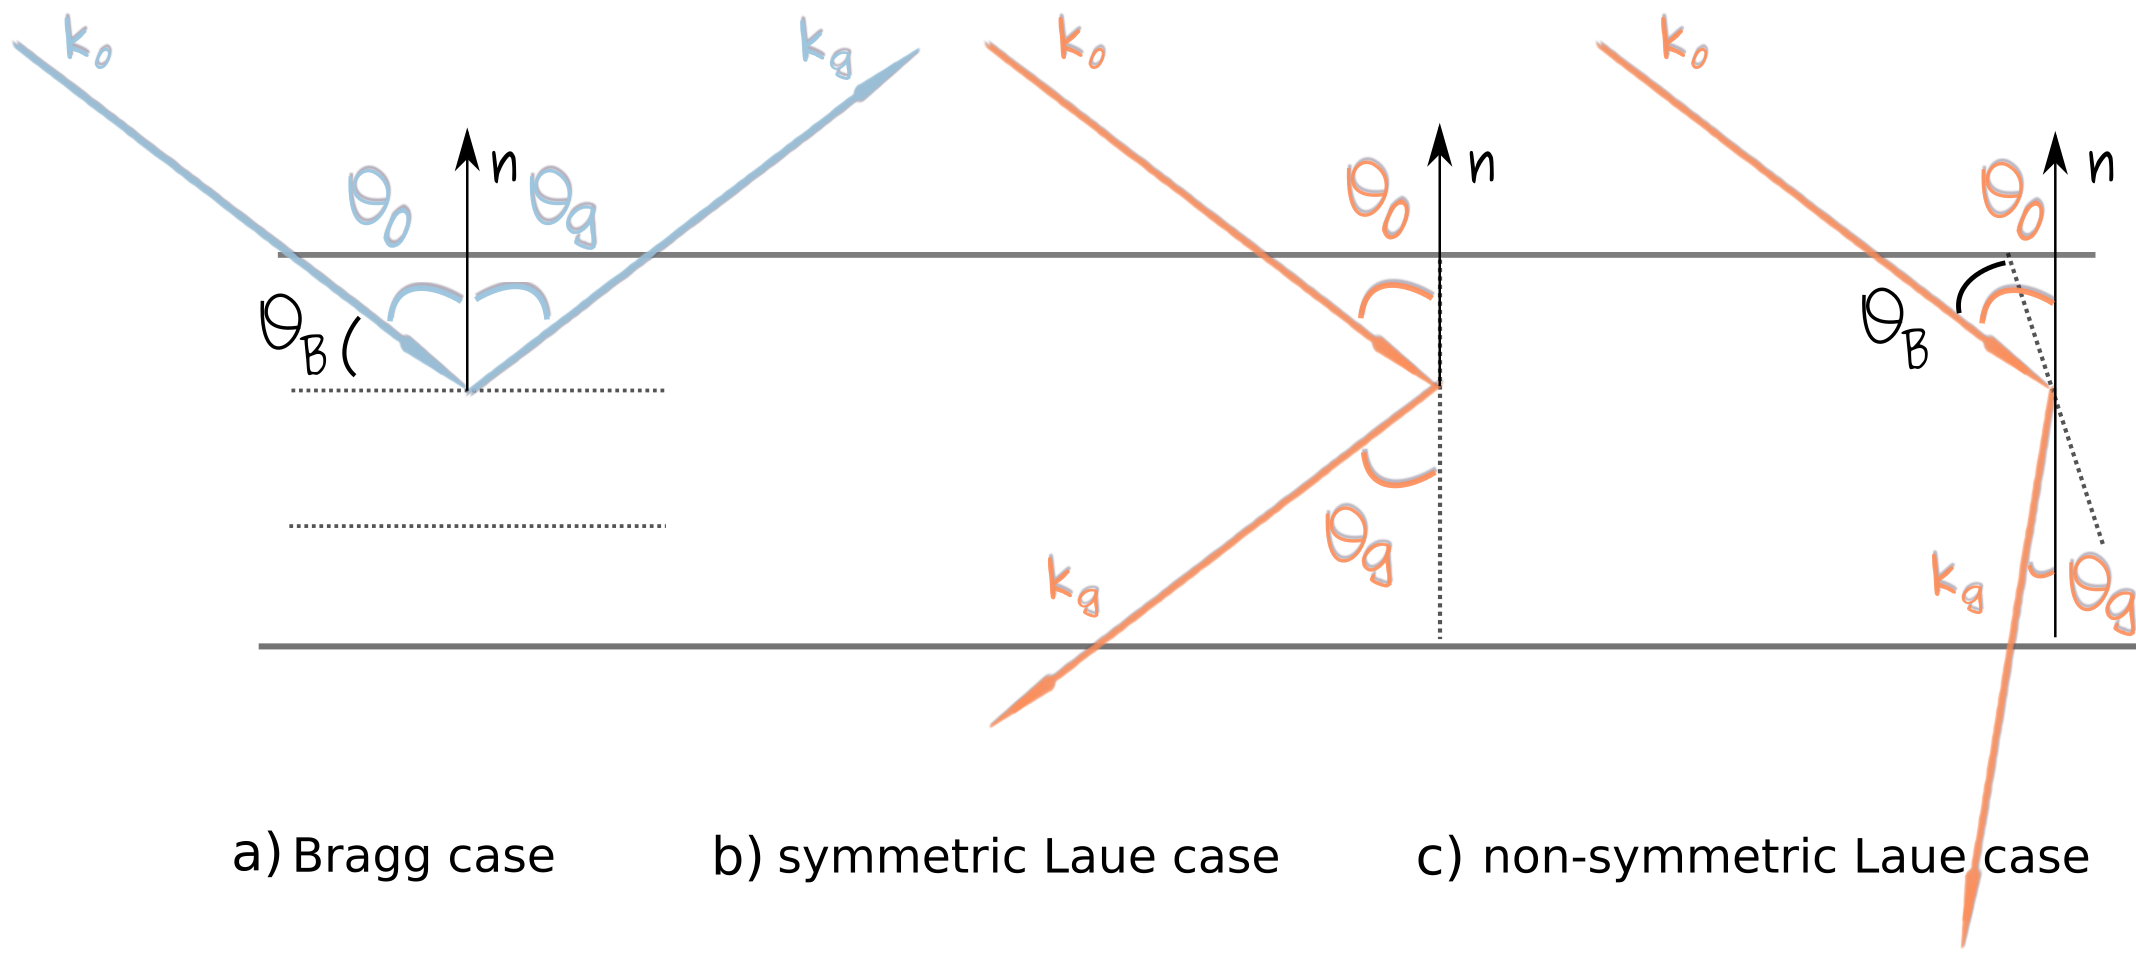
\includegraphics[width=0.92\linewidth]{Figures/BraggvsLaue.png}
\caption[Electron diffraction scattering geometry. ]{Scattering geometry cases relevant in electron diffraction. The angles have been grossly exaggerated. }
\label{Fig:BraggvsLaue}
\end{figure}
%---------

Let us introduce two new angles: $\theta_0$ as the angle between the incident beam direction and the sample normal, $\mathbf{n}$,  and, reversely, $\theta_\mathbf{g}$ as the angle between the diffracted beam direction and the sample normal (see Fig.~\ref{Fig:BraggvsLaue}). 
Depending on the general direction of the diffraction planes with respect to the crystal sample surface, electron microscopists differentiate between:
\begin{itemize}
    \item \emph{symmetric Bragg case} (Fig.~\ref{Fig:BraggvsLaue}~a)) :  when the diffracted beam escapes the sample through the same surface the incident beam entered. This geometry is defined by the film normal being also the normal to the diffracting planes \hkl{hkl}. The relationship between the angles is:
    \begin{equation*}
        \theta_0 =   \theta_\mathbf{g} =\pi/2 -\theta_B.
    \end{equation*}
     \item \emph{symmetric Laue case} (Fig.~\ref{Fig:BraggvsLaue}~b)) : when the diffracted beam escapes from the  bottom of the sample. This geometry is defined by the film normal being parallel to the  diffracting planes \hkl{hkl}.  The relationship between the angles is:
      \[ \theta_0 =   \theta_\mathbf{g} = \theta_B.\]
    \item  \emph{non-symmetric Laue case} (Fig.~\ref{Fig:BraggvsLaue}~c)) : is a generalised form of the one above. There is now  a nontrivial angle between the diffracting planes and the surface normal. The only relationship we can write between the three angles is:
    \[ \theta_0 +  \theta_\mathbf{g} = 2 \theta_B.\]
\end{itemize}
\vspace{-0.5cm}

 The form of dynamical theory commonly used in TEM diffraction contrast description is based on the symmetric Laue case~\cite{Howie61}. This geometry is assumed valid for a large range of diffraction conditions that deviate from the perfect symmetric case.  Whelan and Hirsch~\cite{Whelan57} showed that the angle of a stacking fault\footnote{A stacking fault is a planar defect telling us that for a given set of planes of atoms there is an error in their stacking structure. } introduced in a perfect crystal does not affect two beam dynamical calculations of diffraction intensities. Furthermore, Saldin \etal~\cite{Saldin78} showed that the Darwin equations predict very small errors for a wide range of incident angles when the non-symmetric Laue case is approximated to a symmetric one. A good summary of this discussion was published by Sheinin and Jap~\cite{Sheinin79} who also took the conversation further. They used a Bloch wave formalism to test the limits of this approximation and concluded that for strong beams\footnote{ Strong beams as opposed to weak beam conditions where the deviation from the exact Bragg condition is quite large. More about this on page~\pageref{sec:sg}.} there is no significant difference between the predictions in the symmetric and non-symmetric Laue cases.




%%%%%%%%%%%%%%%%%%%%
\section{Diffraction intensity}
\label{sec:intensity}


We have explored so far the geometrical conditions for constructive interference, \ie diffraction, to occur in a crystal.  But, as we will see on page~\pageref{sec:strucFact}, while a necessary condition, Bragg's law being satisfied is not sufficient for non zero intensity along a given direction. This is because Bragg's law gives us information only about the lattice orientation with respect to the incoming beam direction. However, we are free to decorate this lattice in more than one way, and the motif can end up scattering out of phase with the planes.  

It therefore becomes important to understand the probability of scattering first from a single atom. Bragg's law remains the same for photons, electrons or neutrons even though the Bragg angles can vary greatly, depending, as they are, on the energy of the incoming beam. But the scattering physics and resulting intensity is dependent on the type of incident particle. We have seen in Table~\ref{table:diffractingParticles} on page~\pageref{table:diffractingParticles} that while X-rays interact only with the electron cloud, electrons are scattered by both the cloud and the atom nuclei. In the next pages we will see how to calculate scattering probabilities, \ie \textit{scattering factors},  for a number of common directions in binary group-III nitride systems. 

Next, on page~\pageref{sec:strucFact} we put all atoms on a unit cell and calculate the total scatter probability  as a sum of all their contributions for a given direction. In the process we will introduce the useful mathematical concept of \textit{structure factor} which describes how the positions of the atoms in the unit cell affect the intensity of the diffracted beam. 

 The high energy of the incoming beam simplifies the crystal to the behaviour of isolated spherical point scatterers. The parameters discussed in this sections are important because they constitute the only information we track about the crystal structure when we model electron diffraction. On page~\pageref{sec:ICpotential} we discuss how to calculate a crystal electrostatic potential that takes into account all this directional scattering information. 
 
 Finally, on page~\pageref{sec:SF_GAN}, we calculate the structure factors for a few nitride systems and discuss the systematic absences present in wurtzite. 





%%%
\subsection{X-ray scattering by electron charge density and the X-ray scattering factor}

When a linearly polarised, monochromatic plane-wave X-ray beam is incident upon a stationary atom of atomic number Z, each of its Z electrons will scatter the X-ray waves. The oscillating electric field of the incident X-ray beam excites the individual electrons of mass $m$ and charge $e$ causing them to oscillate at the same frequency as the incident radiation. In turn, the individual electrons, now in the form of accelerated charge, will become a source of spherically radiated X-rays of frequency equal to the incident one. Multiple scattering processes can occur including incoherent scattering or Compton processes but for now we will only consider coherent scattering.


The intensity of a scattered radiation at a distance $r$ from the scattering site of the individual electrons in terms of the incident radiation intensity $I_0$ and the scattering angle $\theta$ is well described by Thomson's equation:
\begin{equation}
I = I_0 \frac{K}{r^2}\sin^2 {\theta},
\end{equation}
which highlights the high directionality of coherent scattering. That is to say, most of the intensity of scattered X-rays will be in the forward direction. In the above equation $K$ is a very small constant given by:
\begin{equation*}
K = \left( \frac{\mu_0}{4 \pi} \right)^2 \times \left( \frac{e^4}{m^2} \right) = 7.9 \times 10^{-30} \si{\meter}^2
\end{equation*}
indicating that in practice scattering effects can become measurable only when a large number of electrons ($ > 10^{23}$) are scattering.

\noindent \begin{minipage}{0.45\textwidth}
In the forward direction, each of the Z electrons will scatter the X-rays beam with an identical phase change of $\pi$ and no destructive interference (see Fig.~\ref{Fig:atomScatter} a)). Scattering in any other direction, $\theta \neq 0$, will result in pathway differences between X-rays scattered by different electrons. The loss of intensity due to destructive interference will translate to a reduced scattered intensity when compared to the forward scattered case (see Fig.~\ref{Fig:atomScatter} b)).
\end{minipage}
\begin{minipage}{0.55\textwidth}
    \centering
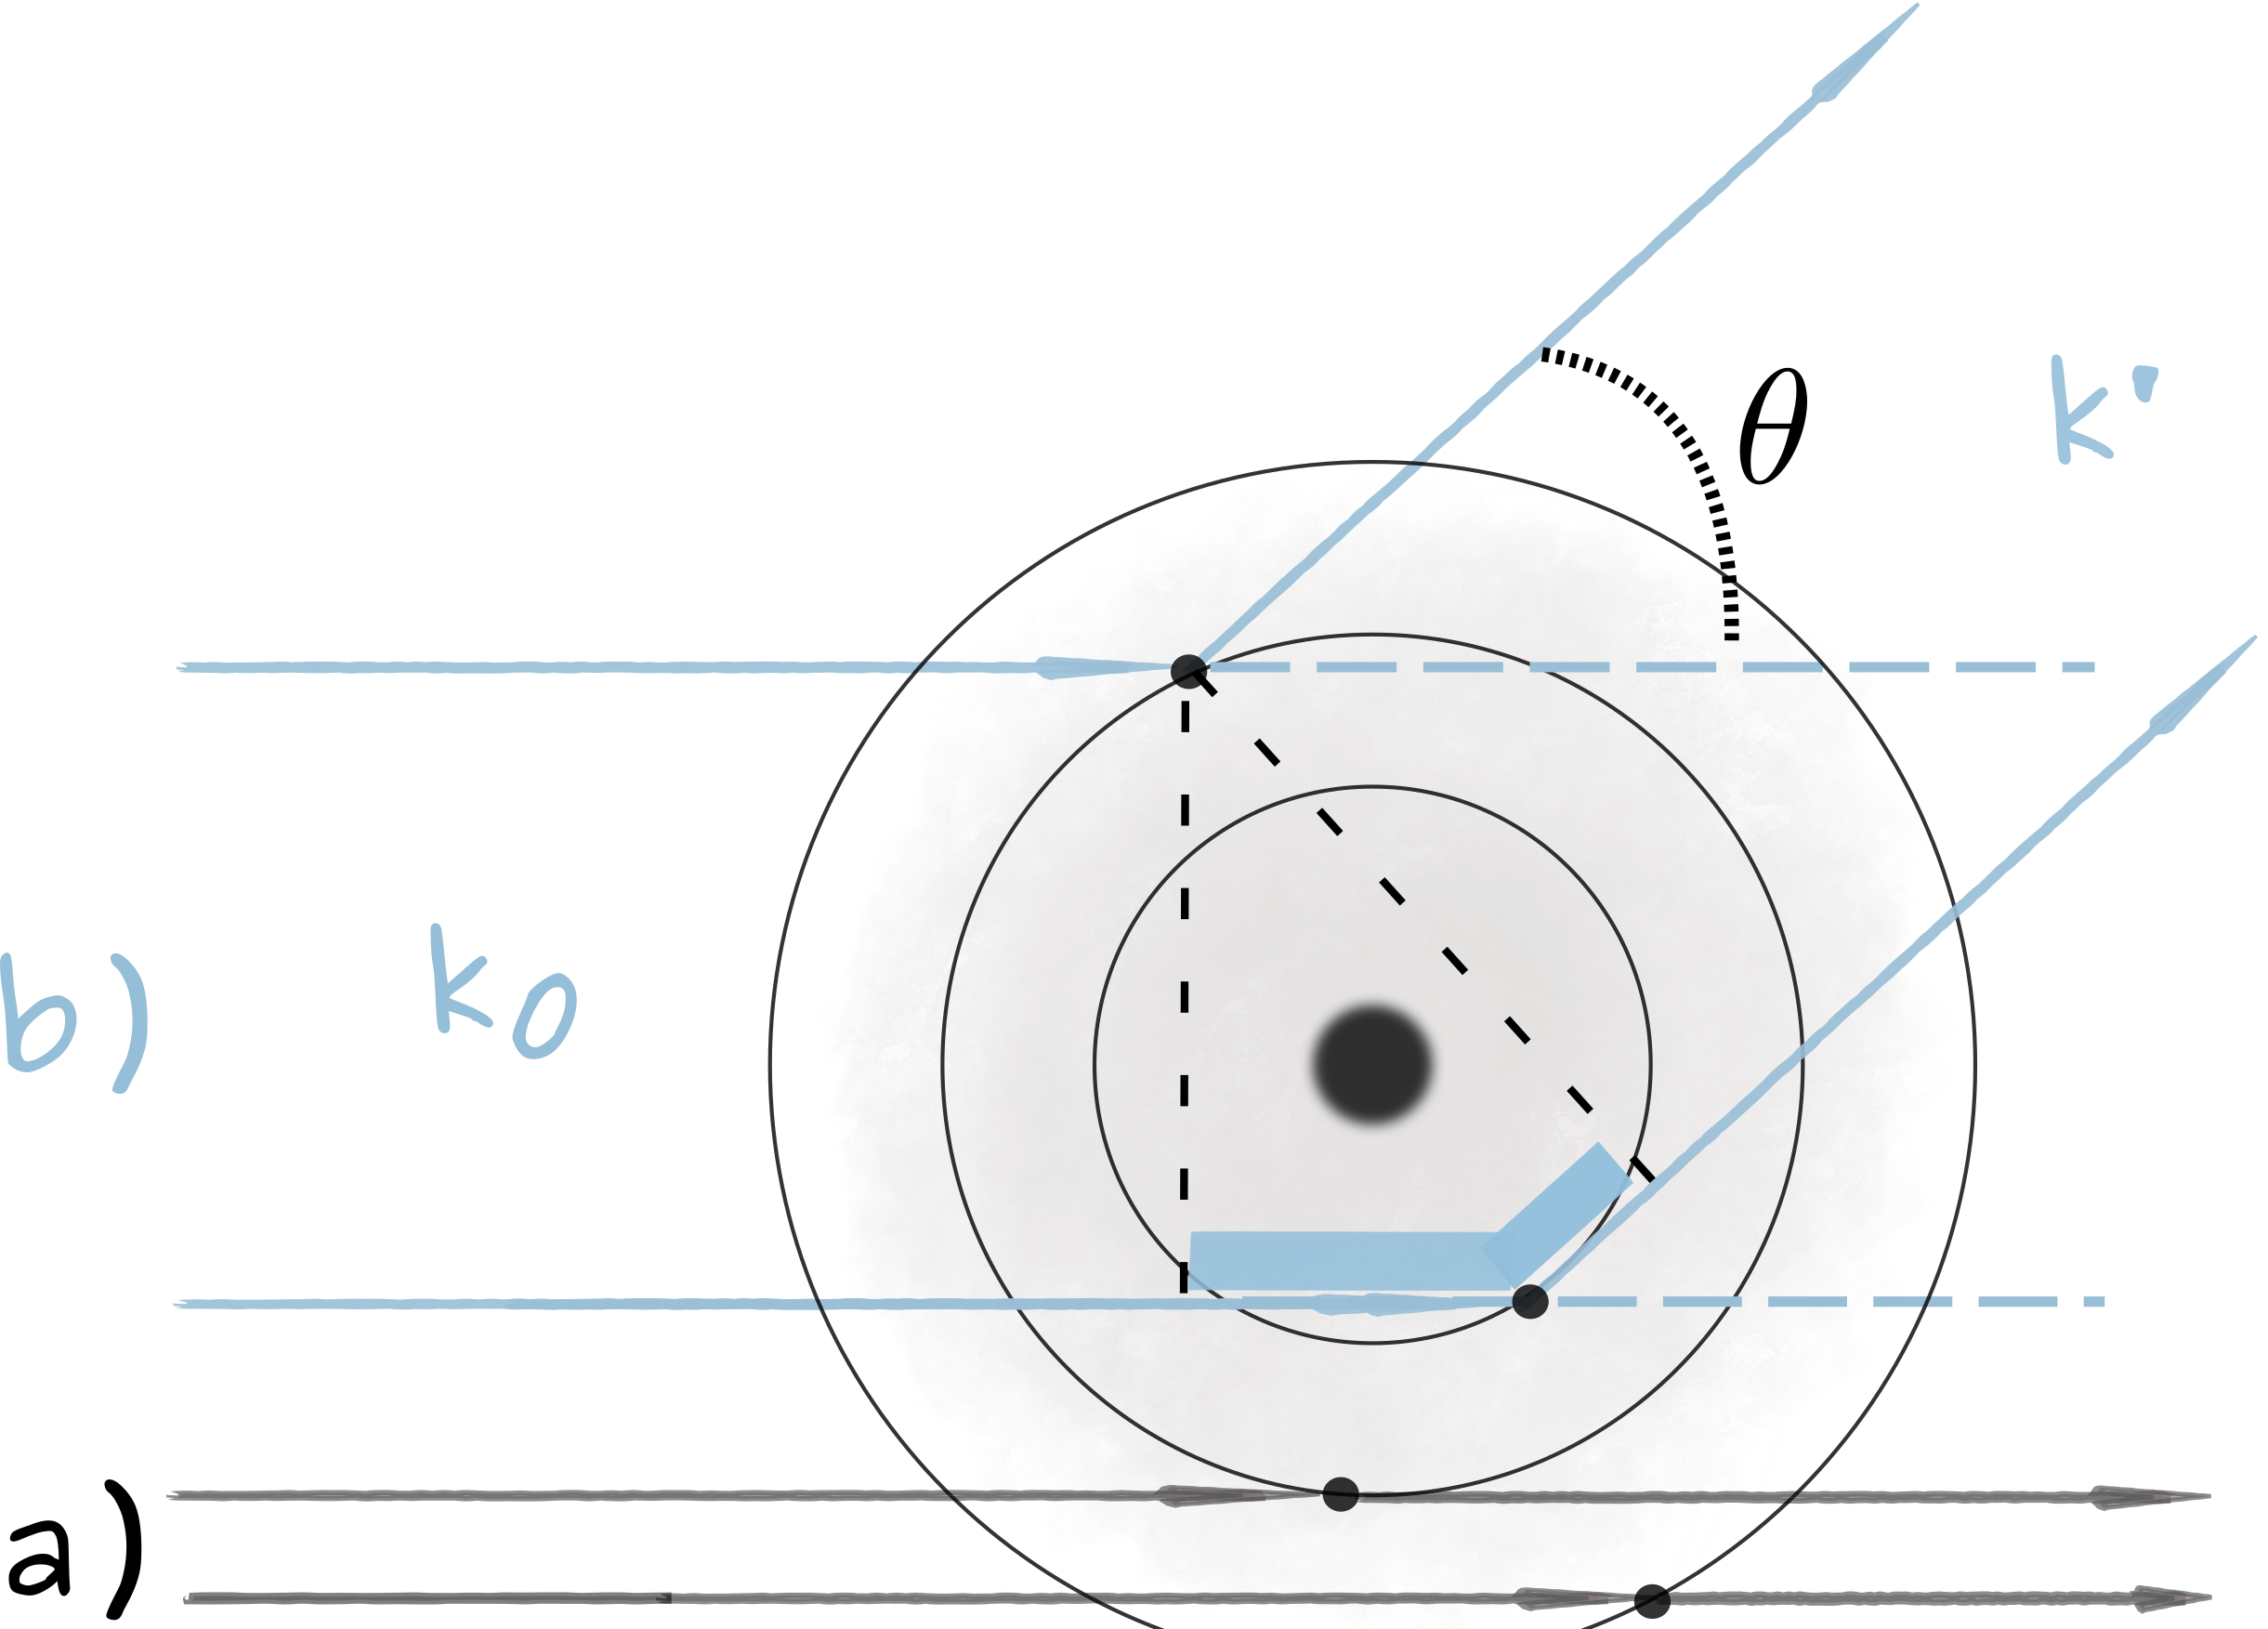
\includegraphics[width=0.7\linewidth]{Figures/atomScatter.png}
\captionof{figure}[Schematic diagram of scattering by an atom.]{Schematic diagram of a) forward scattering and b) scattering by an angle $\theta$. Note the pathway difference marked by thick blue line in b). }
\label{Fig:atomScatter}
\end{minipage}

\hspace{0.5cm}

It is now time to introduce the atomic scattering factor, $f^X$, for a given direction $\theta$ and wavelength $\lambda$ as the ratio of amplitude scattered by an entire atom to the amplitude scattered by only one electron in the same direction. Equivalently, the atomic scattering factor can be thought of as the probability amplitude that the atomic potential of an atom will scatter an incident wave with wave vector $\mathbf{k_0}$ into the direction $\mathbf{k'}$. But this probability is the Fourier transform of the atomic potential that does the scattering, which in the case of incident X-rays is the electron charge density. The \textit{International Tables of Crystallography} ~\cite{IntTableCrysBX} contain tabulated calculated scattering intensity values for all atoms. Since it would be tedious to list the scattering factor values for all possible $\theta$ and $\lambda$, it is often more convenient to list them as curve fitting parameters. The scattering factor fitted function as a function of the variable $s = \sin{\theta}/\lambda$ is then given by:

\begin{equation}
f^X(s) = Z - 41.78214 \, s^2 \, \sum_{i=1}^N a_i e^{-b_i s^2}
\label{eq:xSF}
\end{equation}




\begin{table}
\caption[Doyle \& Turner atomic scattering parameters.]{Doyle \& Turner atomic scattering parameters~\cite{Doyle68} for a few elements. These values were calculated assuming that $s$ is expressed in $\si{\angstrom}^{-1}$. }
\label{table:parX}
\centering
\begin{tabular}{ l l c c c c c c c c }
\toprule
\tabhead{Element} & \textbf{Z} & $a_1$ & \tabhead{$b_1$} & \tabhead{$a_2$} & \tabhead{$b_2$} & \tabhead{$a_3$} & \tabhead{$b_3$} & \tabhead{$a_4$} & \tabhead{$b_4$}\\
\midrule
              N    &    7  & 0.572 & 28.847 & 1.043 & 9.052  & 0.465 & 2.421 & 0.131 & 0.317 \\
              Al   &    13 & 2.276 & 72.322 & 2.428 & 19.773 & 0.858 & 3.080 & 0.317 & 0.408 \\
              Ga   &    31 & 2.321 & 65.602 & 2.486 & 15.458 & 1.688 & 2.581 & 0.599 & 0.351 \\
              In   &    49 & 3.153 & 66.649 & 3.557 & 14.449 & 2.818 & 2.976 & 0.884 & 0.335 \\

\bottomrule
\end{tabular}
\end{table}

Table \ref{table:parX} lists the Doyle-Turner~\cite{Doyle68} $a_i, b_i$ parameters values ($N=4$) for a few group III-nitrides semiconductor elements: N, Al, Ga and In. Note that the values in the table are given assuming $s$ is expressed in $\si{\angstrom}^{-1}$ and $\lambda$ is expressed in  $\si{\angstrom}$. 


The behaviour of the X-ray scattering factor, $f^X_{el.}$, is shown in Figure~\ref{Fig:scatterFactorX} for N, Al, Ga and In. The coloured, vertical lines indicate the $s$ values for the most common planes in wurtzite materials (see Fig.~\ref{Fig:planes}). For instance, the first vertical line (orange), reaching the In line, corresponds to the $s$ value for the c-plane in InN. The scattering factor for $\theta=0$ is the atomic number, and as expected, the curve decreases rapidly with increasing scattering angle (or decreasing wavelength) or, increasing interplanar distance, $d_{hkl}$. 
The code used for these plots and the interactive images can be found in the Jupyter notebook {\tt scatterFactor.ipynb}.

We can observe that the light N atom will scatter fewer X-rays compared to the heavier elements, but at a rate that is consistently comparable to that from Al atoms. We can already conclude that the two species of atoms in AlN will scatter X-rays at comparable rates ($f^X_Al / f^X_N = 1-2 $) and that this ratio depends only lightly on the crystal direction as the two curves are almost parallel. In the \texttt{scatterFactor.ipynb} I also plotted the scattering factors relative to $f^X_{N}$ to make these ratios more readable.  

In contrast, with the increase in mass of the group-III element ($M_{Al}<M_{Ga}<M_{In}$), the rate of scattering becomes significantly different, with Ga scattering X-rays 4-5 times more efficiently than Al, such that we can expect most of the signal to have scattered from the heavy element. Not only this, but for these heavier group-III elements compounds, the more closely packed the planes are (larger $s$) the more the scattering from the heavier element dominates when compared to scattering from N.


%---------
\begin{figure}
    \centering
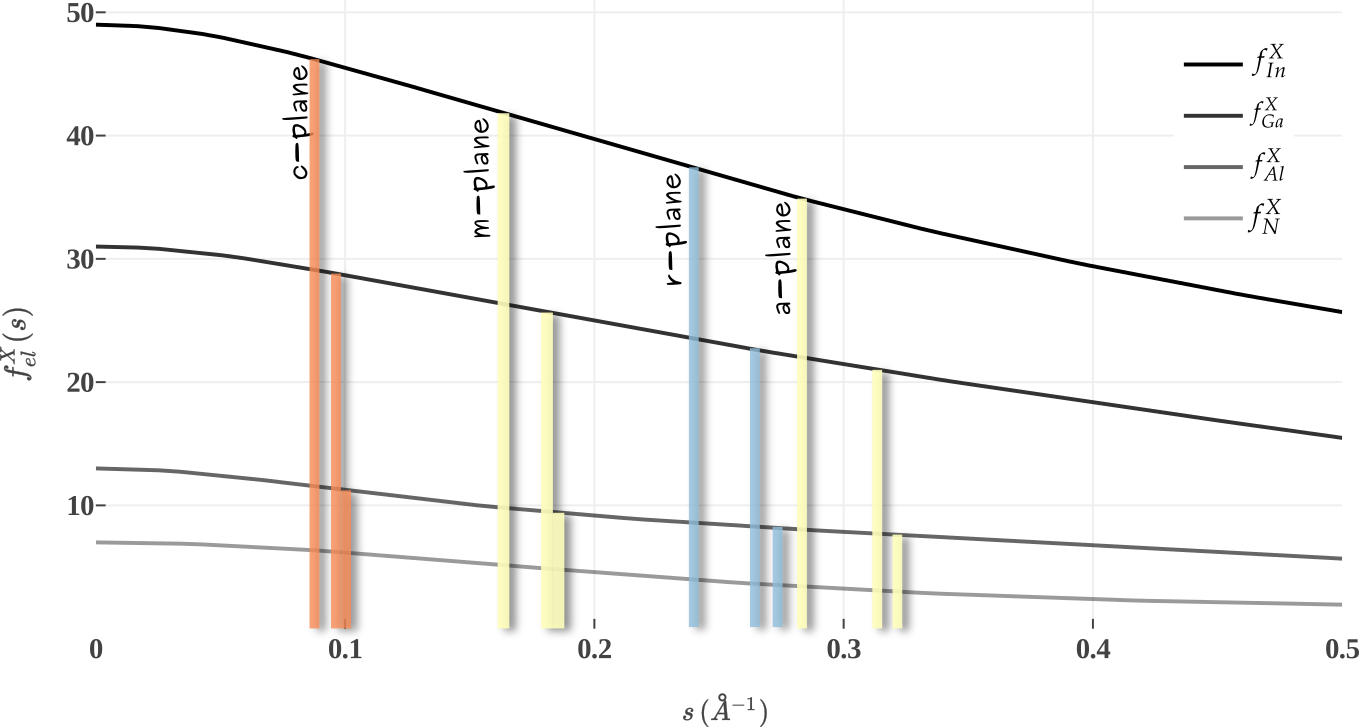
\includegraphics[width=1\linewidth]{Figures/scatterFactorX.png}
\caption[Atomic X-ray scattering factors.]{Atomic X-ray scattering factors for In, Ga, Al and N with superimposed vertical lines indicating the $s$-value for the most common planes in nitrides. The vertical line extend to the group III element curve which makes up the III$_{el}$N compound (\ie InN, GaN and AlN in this order) for which $s_{hkl}$ was computed.}
\label{Fig:scatterFactorX}
\end{figure}
%---------

Note that I only show the curves here for for values of $s\leq$ \SI{0.5}{\angstrom^{-1}} ($d_{hkl}\geq$ \SI{1}{\angstrom}) which is large enough for some of the more common first order reflections. Bear in mind that if we were interested in scattering rates from the higher order reflections we would have to look further to the right on this graph (for AlN $s_{220} = $ \SI{0.64}{\angstrom^{-1}}).





%
\subsection{Electron scattering by a single atom and the electron scattering factor}

As far as the incoming electron beam is concerned, the electrostatic potential $V_{atom}(\mathbf{r})$ of one atom in the specimen is related to its spherically symmetric charge distribution through Poisson's equation:
\begin{equation}
\Delta V_{atom}(\mathbf{r})= - \frac{|e|}{\epsilon_0}\left(\rho _n(\mathbf{r}) - \rho_e(\mathbf{r})\right),
\label{eq:Poisson}
\end{equation}
where $\Delta$ is the Laplacian (second order differential) operator. It will contain a contribution from the point charge nucleus $\rho_n$ and a contribution from the electron cloud charge distribution $\rho_e$.

This does not take us very far since analytical solutions for the electron charge density can only be written for hydrogen. Luckily, the X-ray scattering amplitude calculated on the previous page (Eq.~\ref{eq:xSF}) is the Fourier transform of the electron charge density $\rho_r(\mathbf{r})$ so all that is left to do is to calculate the inverse Fourier transform of the X-ray diffraction amplitude.

We are now ready to define the \textit{atomic scattering factor for an electron} beam $f^e(\Delta \mathbf{k})$, similarly to the case of an incident X-ray beam, as the probability that an incident plane wave with wave vector $\mathbf{k_0}$ is scattered by the atomic potential $V_{atom}(\mathbf{r})$ in the direction $\mathbf{k'}$. Where we introduced the momentum transfer vector $\Delta \mathbf{k}=\mathbf{k'}-\mathbf{k_0}$. Or, equivalently, we can write the probability as the Fourier transform of the atomic potential distribution $V_{atom}(\mathbf{r})$:

\begin{equation}
f^e(\Delta \mathbf{k}) \equiv \iiint V_{atom}(\mathbf{r})e^{-2\pi i \Delta \mathbf{k} \cdot \mathbf{r}} d\mathbf{r}
\end{equation}

Since the atoms studied are part of crystals we can use Bragg's condition, $\mathbf{k'} = \mathbf{k_0}+g$. We will again make use of the useful variable transformation $s = \sin{\theta}/\lambda$, which at the Bragg angle has the magnitude:

\begin{equation}
|\mathbf{s}| = \frac{\sin{\theta}}{\lambda}=\frac{|\mathbf{g}_{hkl}|}{2}=\frac{1}{2 d_{hkl}}.
\label{eq:s}
\end{equation}

Making the approximation that the nuclear charge density can be mathematically written as a delta function of weight Z, we are now ready to inverse Fourier transform all the quantities in Eq.~\ref{eq:Poisson} to obtain:

\begin{equation}
f^e(s)  = \frac{|e|}{16 \pi^2 \epsilon_0 |s|^2} \left[Z-f^X(s) \right].
\label{eq:MB}
\end{equation}

The reader might recognise equation~\ref{eq:MB} to be the Mott-Bethe formula. The use of the variable $s$ defined in Eq.~\ref{eq:s} means that for a given crystal structure the atomic scattering factor is only ``sampled'' at scattering vectors corresponding to half the reciprocal lattice vectors $\mathbf{g}_{hkl}$. It also means that, since for a given crystal structure the magnitude of $\mathbf{s}$ is independent of the wavelength of electrons, the electron scattering factor is independent on the experimental conditions. 

If we use the convenient Doyle-Turner parametrised form of the X-ray scattering factor given in Eq.~\ref{eq:xSF} we can rewrite the Mott-Bethe formula to be:

\begin{equation}
\label{eq:scatterFact}
f^e(s) = 0.04787801\sum_{i=1}^{N=4}a_ie^{-b_is^2},
\end{equation}

This expansion is accurate for values of $s$ up to 20~\si{\nano\meter^{-1}}. Values for the electron scattering factors in a large number of different materials can also be found in the \textit{International Tables for Crystallography}~\cite{IntTableCrysC}. Care must be taken when comparing values from different sources since the factor 0.0478701 can be present or not in the version of Mott-Bethe equation. 

The derivation of Eq.~\ref{eq:scatterFact} made the assumption that the atom is completely still (or at temperature of \SI{0}{K}). Nevertheless, we have already covered in Section~\ref{Sec:DWf} on page~\pageref{Sec:DWf}, that this is a very gross assumption and for any true attempt of understanding scattering we ought to take into account atomic vibrations. We therefore use Eq.~\ref{eq:scatterFactDW} to correct the scattering factor for isotropic, thermal atomic vibrations so we can rewrite the corrected Mott-Bethe formula as:

\begin{equation}
\label{eq:scatterFactDW}
f_T^e(s) = 0.04787801\sum_{i=1}^{N=4} a_i e^{-b_i s^2}  e^{-B_{el.} s^2},
\end{equation}
where $B_{el.}$ is the Debie-Whelar factor for the given element which we calculated on page~\pageref{Sec:DWf} for some of the nitride elements.

Figure~\ref{Fig:scatterFactor_e} plots electron scattering factors (Eq.~\ref{eq:scatterFact}) for Al, Ga, In and N in continuous lines together with the DW corrected versions (Eq.~\ref{eq:scatterFactDW}) at \SI{300}{K} in dashed lines. We can see the overall behaviour is not completely dissimilar from that of X-ray scattering in Fig.~\ref{Fig:scatterFactorX}. See the description for that figure on how to read the vertical lines. The code used for this plot can be found, as well, in the Jupyter notebook {\tt scatterFactor.ipynb}. 


%---------
\begin{figure}
    \centering
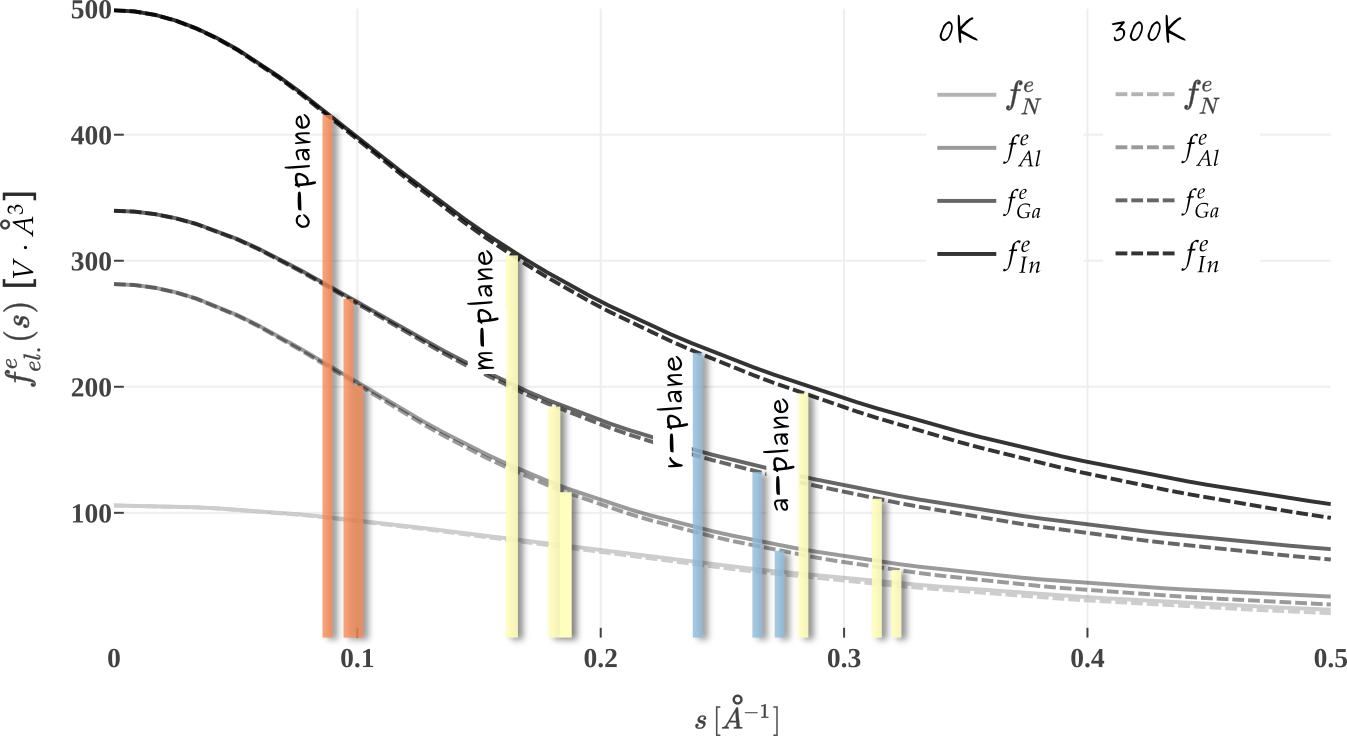
\includegraphics[width=1\linewidth]{Figures/scatterFactor_ecor.png}
\caption[Atomic electron scattering factors.]{Atomic electron scattering factors for In, Ga, Al, N with superimposed coloured lines indicating the most common planes for nitrides (see Fig.~\ref{Fig:planes}). }
\label{Fig:scatterFactor_e}
\end{figure}
%--------- 


As discussed on page~\pageref{table:diffractingParticles} and showcased in Table~\ref{table:diffractingParticles}, electron beams scatter significantly more in matter compared to X-rays which also transpires when comparing the values on the y-axes. This is due both to their smaller wavelengths and the fact that they interact with the entire atom not just the electric field. The added delta function-like nucleus potential makes the electron scattering factor much more sensitive to the direction of scattering and we can see the curve decays more rapidly than in the X-rays case. 


The DW corrections become significant the more the interplanar distances are reduced. That is to be expected since the more comparable the interplanar distance becomes to the spatial range of the atom potential the more the point average position approximation breaks apart. The correction continues to become more significant as we go to higher values of reciprocal interplanar distances ($s_{hkl}$), \eg for higher order reflections. The other factor that affects the correction factor is the size of the atom in the first place, with heavier atoms requiring larger correction factors. We can see that for the chosen range of $s$-values, the correction factor for N is about 1\% and therefore almost indistinguishable in  these figures. For In, however, it becomes close to 10\% especially on the right side of the x-axis. 



%---------
\begin{figure}
    \centering
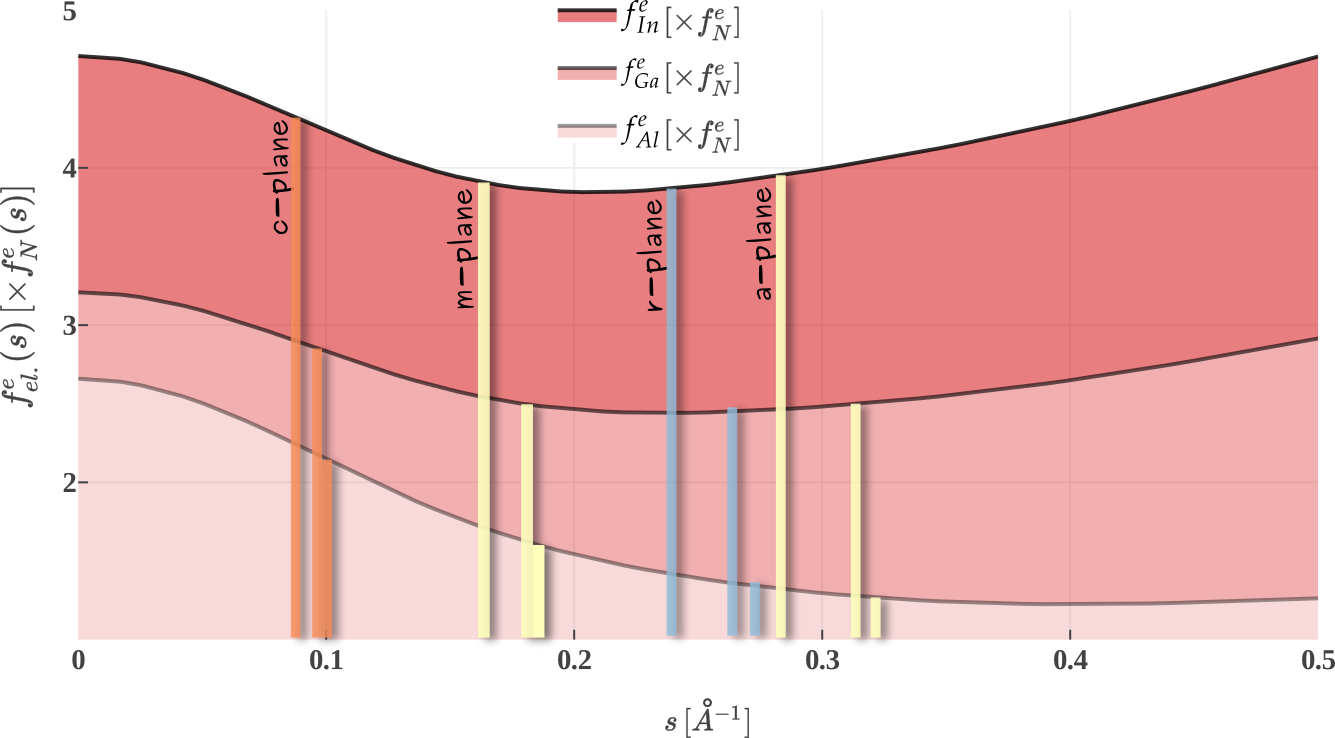
\includegraphics[width=1\linewidth]{Figures/scatterFactor_eRel.png}
\caption[Relative atomic electron scattering factors.]{Relative atomic electron scattering factors for In, Ga, Al in terms of scattering from N atoms. The superimposed coloured lines indicating the most common planes for nitrides are the same as before. }
\label{Fig:scatterFactor_eRel}
\end{figure}
%---------

In Fig.~\ref{Fig:scatterFactor_eRel} I show the same electron scattering factors from Al, In and Ga but this time relative to the scattering factor for N atoms in order to highlight how the rate of scattering changes for different planes in binary compounds. For AlN the electrons scatter 1-3 times more frequently from the Al atoms than from the N atoms. This rate is highly sensitive to the direction of scattering such that for larger interplanar distances (\textit{c}-plane) the scattering intensity is made of up two parts from the group-III element scattering and one part from N. At smaller interplanar distances the scattering from N and Al is almost equal. 


Because the electron scattering factor for N decays faster with $s$ than that for Ga and In, the relative scattering for these heavier group III elements goes up after about $s=$ \SI{0.2}{\angstrom}. Such that at small interplanar distances, \eg higher order reflections, scattering from the heavier element in the compound dominates 3-7 times that from N atoms. 



%
\subsection{Scattering by the unit cell and the electron structure factor}
\label{sec:strucFact}

Now that we know how charged particles scatter from a single atoms and from lattice planes, we can tackle a full unit cell by taking into account the relative positions of all the atoms in it. More practically, we need to address how  we account for the relative phase of scattering from two atoms not belonging to the same family of planes. I'll show here the derivation from \textit{Structure of Materials ...}~\cite{SoM} pg.~298 which uses, as a working example, an atom places in between two planes. 


\noindent \begin{minipage}{0.43\textwidth}
Let us revisit Fig.~\ref{Fig:Bragg}, which I update here in Fig.~\ref{Fig:BraggSF}. Beams 1) and 2), in blue, are scattered in phase since the incident angle $\theta = \theta_B$ satisfies Bragg condition. Let this set of planes be \hkl(100). If we now add an atom at position $r$ such that it lives on the orange plane, let it be \hkl(200), in between the \hkl(100),  let us investigate how much destructive interference will it contribute to the scattered signal when a beam 3), in orange, scatters from it.
\end{minipage} %
\begin{minipage}{0.6\textwidth}
\centering
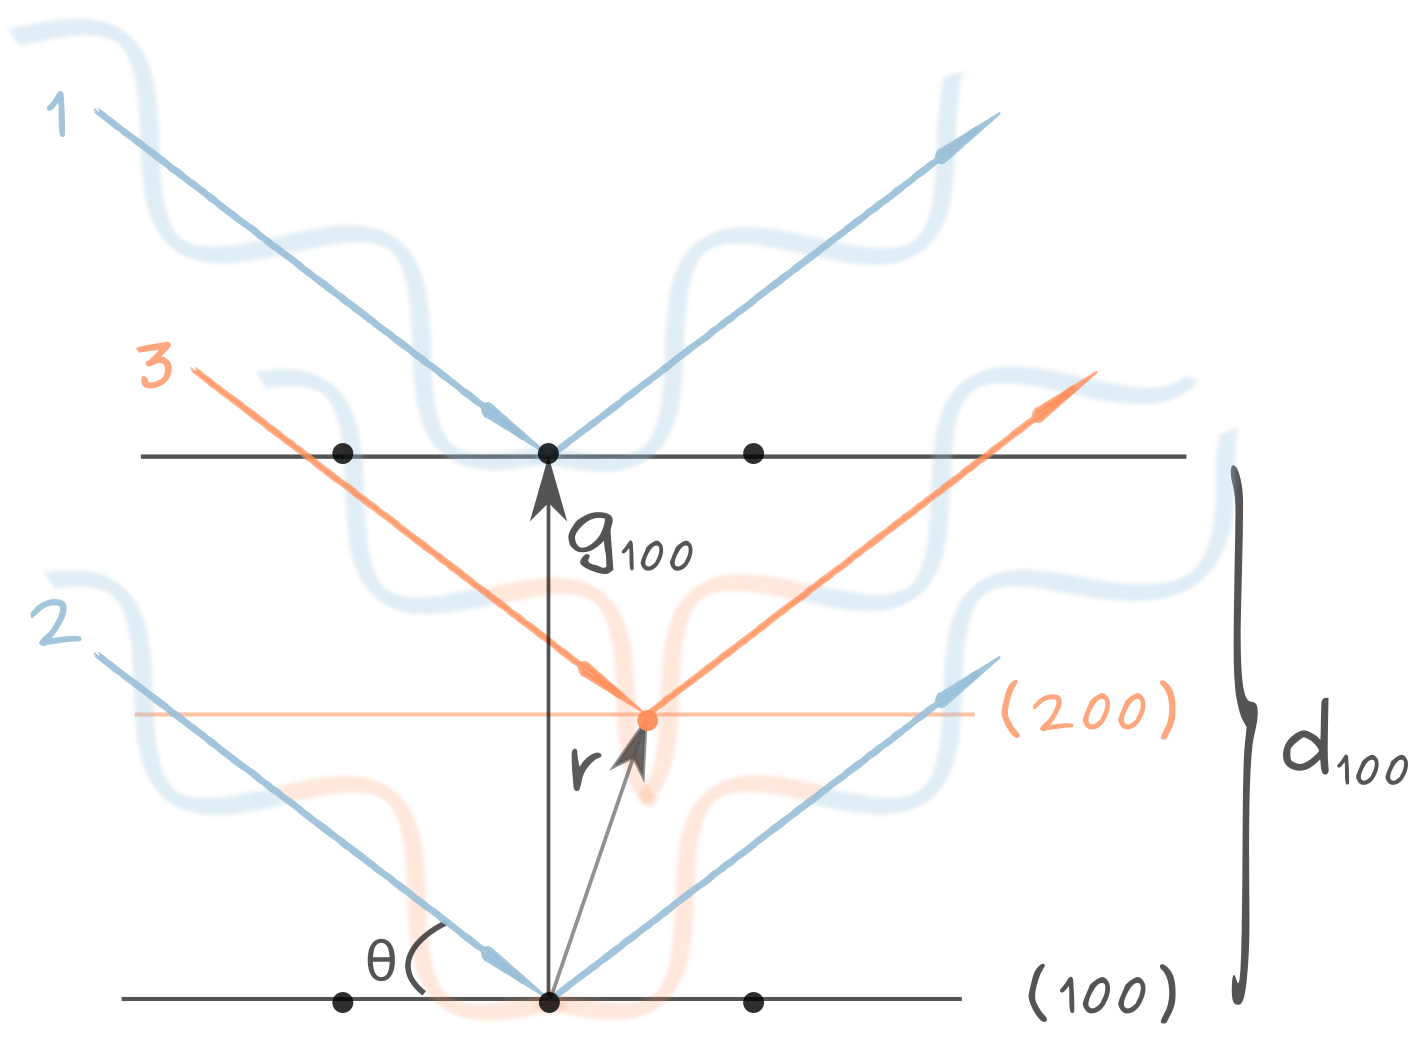
\includegraphics[width=0.87\linewidth]{Figures/BraggSF.png}
\captionof{figure}[What happens to the Bragg's law when we add an atom in between planes?]{What happens to the Bragg's law when we add an atom in between planes? [Based on Fig. 12.4 in~\cite{SoM}]}
\label{Fig:BraggSF}
\end{minipage}

\vspace{0.3cm}

To answer this, section~\ref{Sec:Bragg} on page~\pageref{Sec:Bragg} already prepared us to think about the difference in phase between beams 1) or 3) and beam 2). The path difference between the coherent scattered beams 1) and 2) is a full wavelength $\lambda$. It turns our that the difference in phase between beam 1) and 3) is independent on where on plane \hkl(200) the atoms sits, all that matters is the distance to the planes \hkl(100). For plane \hkl(200) the extra atom sits at a distance $d_{hkl}/2$ from planes \hkl(100). This distance can be written as the projection of vector $\mathbf{r}$ onto $\mathbf{g}_{100}$, \ie $\mathbf{g}_{100} \cdot \mathbf{r}$. We can then transform this distance to a phase by multiplying by $2\pi$:
\begin{equation*}
\phi_{1 \rightarrow 3} = 2\pi \mathbf{r} \cdot \mathbf{g}_{100} = \pi
\end{equation*}
This means the scattered beam 3) will be out of phase with 1) and 2), resulting in destructive interference. And this despite the fact that the Bragg condition is geometrically satisfied for \hkl(100) planes! 

The phase equation above can be generalised to scattering from any atom at position $\mathbf{r}=(x, y, z)$ living outside a set of planes \hkl(hkl):
\begin{equation*}
\phi = 2 \pi \, \mathbf{r} \cdot \mathbf{g}_{hkl} = 2\pi ( hx + ky + lz)
\end{equation*}

We are now ready to write out the full unit cell to the total scattering from planes \hkl(hkl) as the sum over the contributions of all the atoms:
\begin{equation}
\label{eq:scatFactEqS}
F_{hkl} = \sum_{j=1}^{N} f^e_j(s) \, e^{i\phi_j} =  \sum_{j=1}^{N} f^e_j(s) e^{2\pi i \mathbf{r}_j \cdot \mathbf{g}_{hkl}} =  \sum_{j=1}^{N} f^e_j(s) e^{2 \pi i \, (hx_j + ky_j + lz_j)}
\end{equation}
where the index $j$ in the sum goes over all the N atoms in the unit cell and $s=\frac{\theta_{hkl}}{\lambda}$.

We can generalise the sum over all the atoms in the fundamental unit cell, to be the sum over the atoms in the asymmetric unit cell, $N_a$, times a sum over all the equivalent positions of those atoms in the fundamental unit cell (\ie \textit{orbit})\cite{MarcTEM03}. We can write the second sum with the help of the Seitz symbol $(\mathsf{D}|\mathbf{t})$ (see page~\pageref{eq:Seitz} in Appendix~\ref{Chap:Symmetry}):

\begin{equation}
\label{eq:scatFactEq}
F_{hkl} = \sum_{j=1}^{N_a} f^e_j(s) \sum_{(\mathsf{D}|\mathbf{t})} e^{2\pi i  \mathbf{g}_{hkl} \cdot (\mathsf{D}|\mathbf{t})[\mathbf{r}_j] }
\end{equation}



This sum is known as the \textit{structure factor} and, as we have seen in Table~\ref{table:kinVsDyn} it is used in the kinematical model to predict the intensity of diffracted electrons. We will talk about its prediction for nitrides in the following section.

%
\subsection{The structure factor in wurtzite nitrides}
{\label{sec:SF_GAN}}

It is finally time to fill in Eq.~\ref{eq:scatFactEq} or Eq.~\ref{eq:scatFactEqS} the position of the atoms in a wurtzite unit cell, Eq.~\ref{eq:positionGa1} to Eq.~\ref{eq:positionN2} (given on page~\pageref{eq:positionGa1}), and derive some structure factors for a few $\mathbf{g}_{hkl}$ vectors: 
\begin{align}
\begin{split}
\label{eq:scatFactWurzite}
^{wurtzite}F_{hkl} &= f^e_{III_{el}}  \left[(-1)^{2(\frac{h}{3} + \frac{2k}{3})}  + (-1)^{2(\frac{2h}{2} + \frac{k}{3} +\frac{l}{2})} \right] \\
                & + f^e_{N}  \left[(-1)^{2(\frac{h}{3} + \frac{2k}{3} + \frac{3l}{8})}  + (-1)^{2(\frac{2h}{3} + \frac{k}{3} +\frac{7l}{8})} \right] \\
                %%
                &= (-1)^\frac{2h}{3} (-1)^\frac{4k}{3}  \left( f^e_{III_{el}} +   (-1)^\frac{3l}{8} f^e_{N} \right) \left[ 1  + (-1)^{ (\frac{2(h-k)}{3}  + l)}  \right]
\end{split}
\end{align}
where $f^e_{III_{el}}$ is the scattering factor of the group-III element and we made use of the identity  $e^{-i \pi n}=(-1)^n$ in the second step.


Table~\ref{table:Fhkl} shows computed values of $F_{hkl}$ for the three nitride systems discussed so far in a number of orientations. These values are in general complex and I show them here in the Euler notation form $F_{hkl}=|F_{hkl}| e^{i\phi}$ where $|F_{hkl}|$ is the absolute value and $\phi$ the phase.  If the reader is interested in calculating the structure factors for different directions, my script can be found in \texttt{structureFactor.ipynb} and it is just a matter of changing the $h, k, l$ values. In the kinematical diffraction theory, often used in X-ray diffraction predictions, the diffracted intensity is simply:
\begin{equation}
\label{eq:KinInt}
 I_\mathbf{g} = F_\mathbf{g} F^*_\mathbf{g} =|F_\mathbf{g}|^2   
\end{equation}


It is important to acknowledge the limitations of these values since many assumptions were made to obtain them, not the least that the crystals in questions are perfect. If this were the case, perfect semiconductor crystals being a common phenomenon, this entire project would be less worthwhile. The numbers in this tables are to be read as general behaviour, remembering that a different parametrisation would yield slightly different numbers (see chapter 7 in ref.~\cite{TheoryandPractice} for longer discussion).



%
\begin{table}[ht]
\caption[Structure factors for wurtzite nitrides.]{Structure factors, $F_{hkl}=|F_{hkl}| e^{i\phi}$, for a few different planes in wurtzite nitride systems. }
\label{table:Fhkl}
\centering
\begin{tabular}{ l c c | c c | c c }
\toprule
              & \multicolumn{6}{c}{\tabhead{Structure factor  $F_{hkl}$ [\si{\volt \angstrom^3}]}}\\ \cmidrule{2-7}
              & \multicolumn{2}{c}{\tabhead{AlN}} &   \multicolumn{2}{c}{\tabhead{GaN}} &  \multicolumn{2}{c}{\tabhead{InN}}\\ \cmidrule{2-3}  \cmidrule{4-5}  \cmidrule{6-7}
\tabhead{\hkl(hk.l) \hspace{0.2cm}} & \tabhead{$|F_{hkl}|$} & \tabhead{$\phi$} & \tabhead{$|F_{hkl}|$} & \tabhead{$\phi$} & \tabhead{$|F_{hkl}|$} & \tabhead{$\phi$}\\       
\midrule
              \hkl(00.0)   &  774.67 & 0               &  891.01 & 0               & 1209.21 & 0               \\
              \hkl(00.1)   &  0      & 0               &  0      & 0               & 0       & 0               \\
              \hkl(00.2)   &  155.62 & 0.69            &  275.01 & 0.38            & 491.09  & 0.22            \\[0.2cm]
              %a-plane
              \hkl(-21.0)  &  207.82 & 0               &  324.81 & 0               & 505.58  & 0               \\[0.2cm] 
              %m-plane
              \hkl(10.0)   &  193.10 & 3.14            &  261.85 & 3.14            & 386.70  & 3.14            \\
              \hkl(20.0)   &  85.63  & 3.14            & 138.85  & 3.14            & 218.61  & 3.14            \\[0.2cm]
              
              \hkl(20.1)   &  118.03 & -1.08           &  201.02 & -1.28           & 327.02  & -1.37           \\
              \hkl(2-2.1)  &  118.03 & 2.07            & 201.02  & -1.28           & 327.02  & -1.37           \\
              \hkl(-20.-1) &  118.03 & -2.07           & 201.02  & -1.86           & 327.02  & -1.78           \\[0.2cm]
              %r-plane 
              \hkl(1-1.2)  &  52.57  & -2.34           & 105.50  &  -2.76          & 194.67  & -2.92           \\[0.2cm]
              
              \hkl(30.1)   &    0    & 0               & 0       & 0               & 0       & 0               \\

\bottomrule
\end{tabular}
\end{table}
%




Another observation is that the phase remains the same for a family of planes of the same crystal structure regardless of the atoms that populate it and only the magnitude of the structure factor changes. This observation remains true for different multiplicities as well (see \hkl(1-1.0) and \hkl(2-2.0)).

A first observation is that with the increase in the atomic mass of the group-III element, for the same set of planes, the structure factor increases, as we would expect from the scattering factor behaviour. 

% 1) planes in the same family can have different phase
Another observation would be that the scattering factor for planes belonging to the same family is not required to be the same. We can see that for \hkl(20.1) and \hkl(-20.-1) planes  which have the same absolute scattering factor value but do display different phases. This makes sense because for different planes, even those belonging to the same lattice symmetry, the atoms can be arranged at different positions. 


A more subtle observation is that the interplanar distances are no longer a good indicator of the behaviour of the diffraction intensity behaviour (see Eq.~\ref{eq:KinInt}). In this case, the \textit{a-plane} \hkl(11.0) yields a higher scattering factor then \textit{r-plane} \hkl(1-1.2) with lower interplanar distance. This is because some of the scattering on the \textit{r-planes} leads to destructive interference as discussed in the previous section. 


An important note we will address here is the symmetry of the structure factor. For this we will invoke \textit{Friedel's law} and its application to non-centrosymmetric systems~\cite{Serneels73}. It is straightforward that $F_\mathbf{g}=F^*_{-\mathbf{g}}$ which can be rewritten as $F_\mathbf{g} F^*_\mathbf{g}=F^*_{-\mathbf{g}}F_{-\mathbf{g}}$ or $I_\mathbf{g}=I_\mathbf{-g}$. This is Friedel's law and it tells us that the intensity calculated as proportional to the structure factors absolute value will always show inversion symmetry. This is the behaviour seen for planes \hkl(-20.-1) and \hkl(20.1). Nevertheless, for non-centrosymmetric systems, like the ones discussed here, this is not what we expect. More generally, this kinematical description of the diffracted intensity, while suitable for predicting the scattering behaviour from a centrosymmetric system, fails to predict the break in symmetry of the non-centrosymmetric ones.  This is yet another reason why we have to talk in the following sections about dynamical models for the wurtzite systems. 


The last observation we will discuss here is that the structure factor is exactly zero for some of these planes (\hkl(00.2) and \hkl(30.1)) even if we are strictly respecting their Bragg condition. We will talk more \textit{systematic absences} rules below. 


%%%
\subsubsection{Systematic absences }

 Looking at the last form of the equation and keeping in mind that $h,k,l \in  \mathbb{Z}$ we can find the rules for vanishing scattering factors, \ie \emph{extinction criterion}. The square bracket in Eq.~\ref{eq:scatFactWurzite} tells us that there is exactly one condition for the values $h,k,l$ for which the value of the structure factor is zero, namely:
 
 \begin{equation*}
     \frac{2(h-k)}{3} + l  = 2n+1 \, ( = \text{uneven})
 \end{equation*}

For this sum to be uneven the first factor must be an integer, and can only be an even integer and, therefore, the second term must be even. We can then conclude that even when the Bragg condition is satisfied if the following relationships are satisfied simultaneously between the values $h, k, l$ the diffraction intensity will be zero:

\begin{quote}
  \hspace{1cm}  $h-k=3n$ \hspace{0.5cm} AND \hspace{0.5cm} $l=2m+1$
\end{quote}
where $m,n \in \mathbb{N}$. In Table~\ref{table:Fhkl} we have seen that these conditions are met for \hkl(00.1) and \hkl(30.1). 

Alternatively, we can say that for any departure from these conditions the structure factor will be non-zero, \ie \emph{reflection criteria}:
\begin{quote}
  \hspace{1cm}  $h-k=3n+1$ \hspace{0.5cm} OR \hspace{0.5cm} $h-k=3n+2$  \hspace{0.5cm}  OR  \hspace{0.5cm} $l=2m$
\end{quote}

These are, reassuringly, the same conditions given in the \textit{Tables} for the space group $\mathbf{P6_3mc}$ (see page~\pageref{Fig:ITC}).



%
\subsection{Scattering by an infinite crystal }
\label{sec:ICpotential}

We have previously talked about the interaction of a beam of high energy electrons with a crystalline sample as being mathematically represented in the Schr\"{o}dinger's equation by the electron interaction with the sample's electrostatic Coulomb potential $V(\mathbf{r})$. Finding the correct potential for a given crystalline structure is a fundamental problem in solid-state physics usually tackled by so-called first principles methods. These methods are notoriously expensive when solving even small systems since they aim to provide a solution for the many body problem that is the electron-electron interaction of the crystal structure. Fortunately for electron microscopists, the high energy of the incoming beam simplifies the crystal to the behaviour of isolated spherical point scatterers, where each scatterer is a the potential of a single unit cell. 


Since the unit cells live on the lattice, one way to write out an infinite lattice in maths form is as a set of unit-weight delta functions located at the lattice points:
\begin{equation}
\mathcal{L}(\mathbf{r}) = \sum_{u,v,w} \delta(\mathbf{r}-\mathbf{t}_{uvw})= \begin{cases} 1 & \mbox{if }	\exists \, \, u, v, w \in  \mathbb{Z} \mbox{ such that  }  \mathbf{r}=\mathbf{t}_{uvw} \\
																						  0 & \mbox{otherwise }
																							\end{cases}
\end{equation}
where $\mathbf{t}_{uvw} =  u\mathbf{a} + v\mathbf{b} + w\mathbf{c}$ is the translational lattice vector. The lattice points themselves correspond to single unit cells and their own potential is described by the N atoms in the unit cell located at positions $\mathbf{r}_i$:
\begin{equation}
V_{\text{unit cell}}(\mathbf{r}) = \sum_{i=1}^{N} V_{\text{atom}_i}(\mathbf{r}- \mathbf{r}_i)
\end{equation}

The full lattice potential of an infinite crystal is an instance of the unit cell potential at each lattice point. This can be written as the convolution\footnote{ Convolution with a delta function means ``copying" the unit cell potential at the position of the delta function which, here, is every lattice site.} of the single unit cell potential with the area of delta functions potential of the crystal lattice:

\begin{equation}
V_{\text{IC}}(\mathbf{r} ) = V_{\text{unit cell}}(\mathbf{r})  \circledast  \mathcal{L}(\mathbf{r})
\end{equation}

By construction, $V_{IC}(\mathbf{r})$ has the periodicity of the underlying Bravais lattice:
\begin{equation}
V_{\text{IC}}(\mathbf{r} ) = V_{\text{unit cell}}(\mathbf{r} + \mathbf{t}_{uvw} ),  \forall \text{ Bravais lattice vectors } \mathbf{t}_{uvw} = u\mathbf{a} + v\mathbf{b} + w\mathbf{c}.
\end{equation}
This allows us to conveniently expand the potential as a discrete Fourier series.
\begin{equation}
V_{IC}(\mathbf{r} ) = \sum_{\mathbf{g}} V_{\mathbf{g}} \, \mathrm{e}^{\, 2\pi i \mathbf{g}\cdot \mathbf{r}}
\end{equation}
where $V_{\mathbf{g}}$ are the Fourier coefficients of the electrostatic lattice potential corresponding to each set of planes $\mathbf{g}_{hkl}$ in the crystal. 

It is reasonable to choose $V_\mathbf{g}$ to be proportional to $F_\mathbf{g}$ since the structure factor carries the information about directional scattering we want the potential to have (see Appendix A.1 in Ref.~\cite{Rymer70} for demonstration of the reasons):
\begin{equation}
\label{eq:Vg}
    V_\mathbf{g} = \frac{F_\mathbf{g}}{\Omega} = \frac{0.04787801}{\Omega} \sum_{j=1}^{N_a}  e^{-B_{el.} s^2} \sum_{i=1}^{N=4} a^j_i e^{-b^j_i s^2}    \sum_{(\mathsf{D}|\mathbf{t})} e^{2\pi i  \mathbf{g}_{hkl} \cdot (\mathsf{D}|\mathbf{t})[\mathbf{r}_j] }
\end{equation}
 where $\Omega$ is the usual unit cell volume and we made use of Eq.~\ref{eq:scatterFactDW} and Eq.~\ref{eq:scatFactEq}. This implies the units for the Fourier coefficient will be $<$\si{\volt}$>$.
 

%%%%
\subsection{Scattering by finite crystal}

In practice crystals are not infinite, in fact they usually come in rather small sizes. This affects the form of the crystal potential. Mathematically this can be written as multiplication by a shape function which has non-zero value only inside the crystal. The reciprocal lattice points can no longer be represented by delta functions centred at the points but rather should be approximated to be three dimensional objects.  It also means that the diffraction conditions become more relaxed as we can observe diffraction behaviour even when slightly off the Bragg angle.


\subsubsection{The deviation parameters \texorpdfstring{$\mathbf{s}_g$}{sg}}
\label{sec:sg}

\begin{figure}[ht]
    \centering
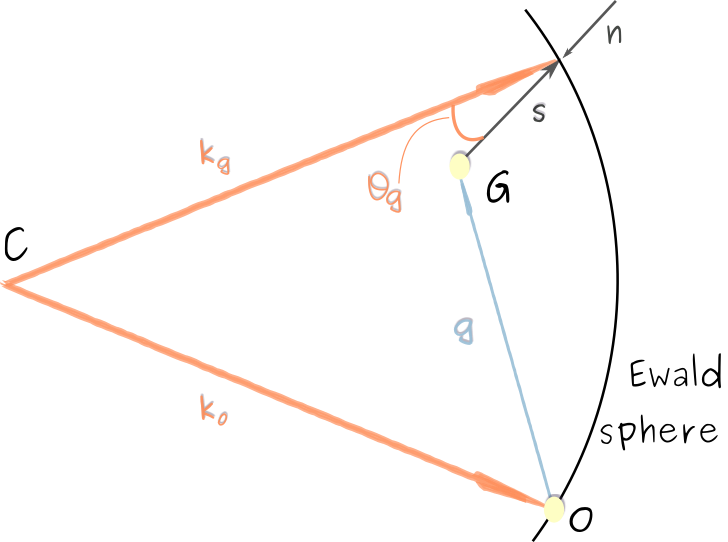
\includegraphics[width=0.52\linewidth]{Figures/EwaldSpheresg.png}
\caption[Ewald sphere construction for a positive deviation parameter $s_g$.]{Ewald sphere construction for a positive deviation parameter $s_g$. $\mathbf{n}$ is the normal to the foil. }
\label{Fig:Ewaldsg}
\end{figure}
%---------

It, therefore,  becomes important to quantify the deviation from the Bragg condition since it is a core parameter in diffraction. For a thin foil the shape of the reciprocal lattice point becomes that of a relrod with one dimension of interest: $\vb{s}=s \vb{n}$. If we redraw Fig.~\ref{Fig:Ewald} and allow a lattice point at distance $\mathbf{s}$ from the Ewald sphere in the direction of the lattice normal to contribute to diffraction we would end up with Fig~\ref{Fig:Ewaldsg}. We can rewrite the Bragg condition ( Eq.~\ref{eq:Bragg1} on page  page~\pageref{sec:Ewald}) as:
\begin{equation}
    \mathbf{k}_{g}- \mathbf{k}_0 = \mathbf{g}+\mathbf{s},
\end{equation}
such that the vector $\mathbf{g} +\mathbf{s} $ is now on the Ewald sphere. Rewriting  Eq.~\ref{Eq:recBragg} with this bit of information:
\begin{equation*}
(\vb{g}+\vb{s}) \cdot(2\vb{k}_0 + \vb{g} + \vb{s}) =0
\end{equation*}

From this we can obtain the length of the vector $\vb{s}$ which is usually repackaged in the following form:
\begin{equation*}
    s + \frac{s^2}{2 |\vb{k}_0 + \vb{g}|\cos{\theta_g}} = \frac{-\vb{g} \cdot(2\vb{k}_0+\vb{g})}{2 |\vb{k}_0 + \vb{g}|\cos{\theta_g}} =\mathbf{s}_g
\end{equation*}
where $\mathbf{s}_g$ is known as the \textit{deviation parameter} and $\theta_g$ is the angle between the normal to the plane and $\vb{k}_g$. I will rewrite $\vb{s}_g$  in a final form that would become useful later:

\begin{equation}
\label{eq:sg}
    \vb{s}_g = \frac{k_0^2 - k_g^2}{2|\vb{k}_g |\cos{\theta_g}}.
\end{equation}






%
\subsection{Treatment of absorption} 
 \label{sec:absorbtion}
The discussion so far applies to perfectly elastic events. However, in real applications, electrons will have non-zero probability to lose energy during scattering events, what we call inelastic scattering processes. These electrons will not travel in the direction predicted by Bragg's equation but contribute to the image in the form of background instead. 
 
In the absence of absorption the potential of the crystal will be a real value. In order to account for loss of electrons from the diffraction signal to inelastic scattering processes a complex optical potential can be introduced~\cite{Gevers66}:
\begin{equation}
\label{eq:Vc}
V_c(\mathbf{r}) = V + i W = \sum_{\mathbf{g}} V_{\mathbf{g}} \, \mathrm{e}^{\, 2\pi i \mathbf{g}\cdot \mathbf{r}} + i \sum_{\mathbf{g}}W_{\mathbf{g}} \, \mathrm{e}^{\, 2\pi i \mathbf{g}\cdot \mathbf{r}}
\end{equation}
where the \textit{absorption Fourier coefficient}, $W_\mathbf{g}$, can be shown to have a form similar to that of $V_\mathbf{g}$ in Eq.~\ref{eq:Vg} where the scatter factor $f^e(s)$ is replaced by an absorptive factor $f'(s)$. The absorptive factor can also be parametrised,  this time using the Weickenmeier and Kohl's parametrisation~\cite{Weickenmeier91}. This formula I did not implement, but it can be found as part of \textit{EMsoft}~\cite{EMsoft} in \texttt{CalcUcg.f90}. 





%%%%%%%%%%%%%%%%%%%%%%%%%%%%
\section{Darwin-Howie-Whelan equations}
\label{sec:DHW}
In this chapter we have alluded a few times at the limitations of the kinematical model and promised to explore a more robust model: the dynamical model. The dynamical model has, in fact, a long history and diverged into versions optimised for different applications. A few of these are given in Table~\ref{table:DynModels}.

\begin{table}[h]
\caption{Various dynamical models used in electron diffraction.}
\label{table:DynModels}
\centering
\begin{tabular}{ l l l }
\toprule
\tabhead{Model} & \tabhead{Based on } & \tabhead{Application} \\       
\midrule
              Bethe's~\cite{Bethe28}                &  eigenvalue equation     & \begin{minipage}{40mm}intensity of diffraction patterns \end{minipage}\\[4mm]
              Cowley-Moddie's~\cite{Cowley57}       &  multi-slice approach    & single crystal TEM                \\[4mm]
              Howie-Whelan~\cite{Howie61}           & \begin{minipage}{35mm}simultaneous differential equations \end{minipage} & diffraction contrast   \\[4mm]
              Van Dyck~\cite{VanDyck80}   &  real space approach  & \begin{minipage}{40mm}improved accuracy on the multi-slice method            \end{minipage}               \\

\bottomrule
\end{tabular}
\end{table}


For my intents and purposes, \ie diffraction intensity and contrast predictions, I will explore only the Howie-Whelan method (HW) in this work since the addition of dislocation strain is more straightforward than in the other models. For now we will focus on its predictions in a perfect crystal. Howie and Whelan followed Bethe's approach developed for the Bragg case in a perfect crystal with no absorption and generalised it. For this they needed to find the form of the wavelength of the diffracting particles as they travel in the crystal potential, \ie solve Schr{\"o}dinger equation. The time independent Schr{\"o}dinger equation can be written for an electron wavefunction $\Psi$ of energy $eE$ in a periodic crystal potential $V(\mathbf{r})$ in the form known as the Helmholtz equation as:
\begin{equation}
\label{eq:SE}
\Delta \Psi(\mathbf{r}) + \frac{8 \pi^2 m e}{h^2}\left[ E + V(\mathbf{r})\right]\Psi(\mathbf{r}) = 0,
\end{equation}
where $m$, $e$, $h$ are the usual constants and $\Delta$ is the Laplace operator standing for:
\begin{equation*}
\Delta \Psi = \frac{\partial^2 \Psi}{\partial x^2} + \frac{\partial^2 \Psi}{\partial y^2} + \frac{\partial^2 \Psi}{\partial z^2}.
\end{equation*}
The meaning of $\Psi$ is taken here to be that the value $\Psi \Psi^* d\tau$ is the probability of finding the electron in the volume $d\tau$. 

Outside the crystal, where the potential term can be taken to be zero, the solution to the equation above will be in the form of a plane wave (see page~\pageref{sec:wave}): $\psi_0(\vb{r}) = e^{2\pi i \vb{k}_0 \cdot \vb{r}}$. Inside the crystal, the electrons are diffracted and follow a direction $\vb{k}_g=\mathbf{k_0} + \mathbf{g}$ for every reciprocal lattice point $\vb{g}$ on the Ewald sphere. The general solution to the equation above must then be a superposition of plane waves, one for each direction predicted by Bragg's law. 
\begin{equation}
\label{eq:psiBragg}
    \Psi(\mathbf{r})= \sum_\mathbf{g} \psi_\mathbf{g} e^{2\pi i \mathbf{k}_g  \cdot \mathbf{r}},
\end{equation}
where $\psi_\mathbf{g}$ is the complex amplitude of the Bragg plane wave $\mathbf{g}$ and is the unknown to be determined.


The crystal potential $V(\mathbf{r})$ can be taken to have the form in Eq.~\ref{eq:Vc}. It is useful at this point to separate the zero-frequency real component $V_0$ out of the Fourier series as it represents the crystal's mean inner potential and a constant independent of the diffracting planes. This positive potential accelerates the electrons as they enter the crystal in a phenomenon known as \textit{refraction}\footnote{ This is equivalent to the decrease in the speed of light as it enters a medium with a refractive index larger than that of vacuum.}.
\begin{equation}
\label{eq:V0}
V(\mathbf{r}) + i W(\mathbf{r}) = V_0 + \sum_{\mathbf{q}\neq 0} V_{\mathbf{q}} e^{2 \pi i \mathbf{q} \cdot \mathbf{r}} + i \sum_\mathbf{q} W_{\mathbf{q}} e^{2 \pi i \mathbf{q} \cdot \mathbf{r}}.
\end{equation}
In the above we have changed the label of the general reciprocal lattice vector $\vb{g}$ to $\vb{q}$ in order to differentiate it from the reciprocal space lattice vector $\vb{g}$ in Eq.~\ref{eq:psiBragg}.


We can also  write out the wave vector of the incident electron beam corrected for refraction by the mean inner potential $V_0$:
\begin{equation*}
 |\mathbf{k_0}|^2 = k_0^2  = 2me(E+V_0)/h^2
\end{equation*}

In preparation for the substitution of Eq.~\ref{eq:V0} in Eq.~\ref{eq:SE} we separate the term $V_0$ using the above identity and add the following shorthand notation:

\begin{equation*}
U(\mathbf{r}) + iU'(\mathbf{r}) = \frac{2me}{h^2}\left\{ \sum_{\mathbf{q}\neq 0} V_{\mathbf{q}} e^{2 \pi i \mathbf{q} \cdot \mathbf{r}} + i \sum_{\mathbf{q}} W_{\mathbf{q}} e^{2 \pi i \mathbf{q} \cdot \mathbf{r}}\right\}
\end{equation*}



Substituting \ref{eq:psiBragg} and \ref{eq:V0} in the master equation \ref{eq:SE} and after some maths we get the following:
\begin{equation*}
\label{eq:almost}
\sum_\mathbf{g}\left\{ i \mathbf{k_g} \cdot \nabla \psi_\mathbf{g}  + \pi \left(k_0^2 - |\mathbf{k}_g|^2\right) \psi_\mathbf{g} \right\} e^{2\pi i\mathbf{k}_g \cdot \mathbf{r}} =
-\pi \sum_\mathbf{q}\sum_\mathbf{g} [U_\mathbf{q} + iU'_\mathbf{q}]\psi_\mathbf{g} e^{2\pi i(\mathbf{q}+\mathbf{k}_g)\cdot \mathbf{r}} 
\end{equation*}

Van Dyck~\cite{VanDyck76} has shown that the second order derivative of the complex amplitude $\psi_{\vb{g}}$ is negligible for high energy electrons and we have dropped it here. This is known as the \textit{high-energy approximation} and Van Dyck showed that it holds for penetration depths up to a few hundred nanometres, depending on the average atomic number of the atoms in the crystal. For TEM high energy electrons, Howie~\cite{Howie61} ignores the first derivative, $\nabla \psi_{\vb{g}}$ as well, but we will keep it.

Let us have a closer look at the $\vb{k}_g \cdot  \nabla \psi_\mathbf{g} $ term in the Eq.~\ref{eq:almost} above. This term can be read as the directional derivative of the Bloch wave $g$ in the direction $\vb{k}_g$ when in perfect Bragg condition. This means we can reduce the grad operator to only one derivative with no loss of information.  We will assign $z_{beam}$ to be the electron beam propagation direction and can be write the dot product as:
\begin{equation*}
\mathbf{k}_g \cdot \nabla \psi_\mathbf{g} = \left| \mathbf{k}_g \right| \, \frac{d \psi_\mathbf{g}}{dz_{beam}} \cos{\theta_B}.
\end{equation*}



We have to make one final substitution in Eq.~\ref{eq:almost}, a trick one. In the second term of this equation $\vb{q}$ stands for a general reciprocal vector which could be replaced by $\vb{q} = \vb{g'}-\vb{g}$ for instance. This has the effect of changing the variable of the sum from $\sum_{\vb{q}}$ to $\sum_{\vb{g'}}$. The right hand side in Eq.~\ref{eq:almost} becomes:

\begin{equation*}
    RHS = -\pi \sum_\mathbf{g}\sum_\mathbf{g'} [U_{\mathbf{g'}-\vb{g}} + iU'_{\mathbf{g'}-\vb{g}}]\psi_\mathbf{g'} e^{2\pi i(\mathbf{k}_g)\cdot \mathbf{r}}
\end{equation*}
where we also interchanged the variables $\vb{g}$ and $\vb{g'}$.
 
Both terms look now like a Fourier expansion with the same basis and the same number of terms. From the properties of Fourier series (see page~\pageref{sec:Fourier}) we know that the the only way this is true is if the individual terms are equal to each other. Writing the equation above for  every $\vb{g}$ term in the sum and after some reordering we end up with:

\begin{equation*}
     \frac{d \psi_\mathbf{g}}{dz_{beam}} - 2 \pi  i \frac{k_0^2 - k^2_g }{ 2|\vb{k}_g| \cos{\theta_B} } \psi_{\vb{g}} = i \pi \sum_{\vb{g}'} \frac{U_{\vb{g}-\vb{g}'} + i U'_{\vb{g}-\vb{g}'} }{|\vb{k}_{g'}|\cos{\theta_B}}\psi_{\vb{g}'}.
\end{equation*}

This form already tells us that that the change in amplitude of a diffracted wave, $\psi_{\vb{g}}$, with penetration depth in the crystal, $z_{beam}$, depends on its current value, $\psi_{\vb{g}}$, but also the amplitudes of all the other waves, $\psi_{\vb{g}'}$,  that satisfy the Bragg condition. The complex electrostatic potential on the right hand side determines how strongly the excited waves are coupled to each other. 

The second term on the left hand side in the equation above reminds us of the form of the deviation parameter, $\vb{s}_g$, given in Eq.~\ref{eq:sg} on page~\pageref{eq:sg}. The different angle showing up here ties in the discussion on page~\ref{Fig:BraggvsLaue}. Only for a symmetric Laue geometry we can replace $\theta_B=\theta_g$. Nevertheless, the error in approximating a non-symmetric Laue case to a symmetric Laue case is not significant for strong beams. 

\begin{equation*}
     2 \pi  i \frac{k_0^2 - k^2_g }{ 2|\vb{k}_g| \cos{\theta_B} } \psi_{\vb{g}} = 2 \pi i \vb{s}_g   \psi_{\vb{g}}
\end{equation*}

Tilting or rotating the sample moves the Ewald sphere and with it the distance between the reciprocal lattice point and the sphere in the direction normal to the sample, \ie $\vb{s}_g$. For a set of diffracted waves only two non-collinear deviation parameters are independent of each other. But these independent parameters, which affect directly the diffraction behaviour, are experimental variables set by the microscope operator and while easy to determine in a TEM, are, unfortunately, complete unknowns to the SEM operator. 

\paragraph{Extinction distance and absorption length}\mbox{}\\


We will introduce one final substitution. Dimensional analysis tells us that since the first term in the equation has units of reciprocal length so must have the last term. Whenever a term in an equation ends up having simple units, physicists will go and give it a name. In this case they split it in two and named the first term \textit{extinction distance}, $\xi_{\vb{g}-\vb{g}'}$, and the second term \textit{absorption length}, $\xi'_{\vb{g}-\vb{g}'}$, defined in terms of the Fourier coefficients of the real and imaginary parts of the lattice potential as follows:
\begin{equation}
    \frac{1}{\xi_{\vb{g}-\vb{g}'}}\equiv \frac{|U_{\vb{g}-\vb{g}'}|}{|\vb{k}_{g'}|\cos{\theta_B}}
\end{equation}
\begin{equation}
    \frac{1}{\xi'_{\vb{g}-\vb{g}'}}\equiv \frac{|U'_{\vb{g}-\vb{g}'}|}{|\vb{k}_{g'}|\cos{\theta_B}}
\end{equation}
where we used the fact that the complex Fourier coefficients of the electrostatic lattice potential can be written in terms of their modulus and phase angles, $\theta_\textbf{g}$ and $\theta'_\textbf{g}$:
\begin{equation}\label{eq:theta_g}
    U_{\mathbf{g'}-\vb{g}} =  |U_{\mathbf{g'}-\vb{g}}| e^{i \theta_{\textbf{g} - \textbf{g'}}}; \quad \quad \quad U'_{\mathbf{g'}-\vb{g}} =  |U'_{\mathbf{g'}-\vb{g}}| e^{i \theta'_{\textbf{g}- \textbf{g'}}}.
\end{equation}



With the help of all these substitutions, we can finally write out the general form of the multibeam Darwin-Howie-Whelan equations~\cite{Howie61} which describe the change in amplitude of electron diffracted beam with distance travelled inside the crystal:
\begin{equation}
\label{eq: multiDHW}
     \frac{d \psi_\mathbf{g}}{dz_{beam}} - 2 \pi  \vb{s}_g \psi_{\vb{g}} = i \pi \sum_{\vb{g}'} \left( \frac{ e^{i \theta_{\textbf{g}- \textbf{g'}}}}{\xi_{\vb{g}-\vb{g}'}} +i\frac{ e^{i \theta'_{\textbf{g}- \textbf{g'}}}}{\xi'_{\vb{g}-\vb{g}'}}\right) \psi_{\vb{g}'}.
\end{equation}



%%%
\subsection{The two beam case}

In the previous section, we started with a form of the Schr{\"o}dinger's equation describing the electron wavefunction in a periodic, crystal potential. Using Bragg's law we expanded the wavefunction in plane waves and, separately, we Fourier expanded the complex crystal potential. The high energy approximation was applied. We equated the individual harmonics terms in the Fourier expansion. We argued that the non-symmetric Laue geometry can be approximated with good confidence to the symmetric Laue case. We introduced the deviation parameter and the extinction distance and absorption length in the equations. Finally, we ended up with the multi beam form of the Howie-Whelan equations. 

We will look now at the two beam case, when there is only one strong diffracted beam dominating diffraction behaviour,  namely $\psi_{\mathbf{g}}$ in addition to the incident $\psi_{\vb{0}}$. Equation~\ref{eq: multiDHW} becomes:

\begin{equation}\label{eq:twobeam1}
\begin{alignedat}{6}
\dfrac{d\psi_{\mathbf{0}}}{dz_{beam}} &  & \quad = \quad
& -\frac{\pi}{\xi'_\mathbf{0}}\psi_\mathbf{0} & 
\quad + \quad & i \pi \left( \frac{e^{i \theta_{-\mathbf{g}}}}{\xi_{-\mathbf{g}}} + i \frac{ e^{i \theta'_{-\mathbf{g}}}}{\xi'_{-\mathbf{g}}} \right) \psi_{\mathbf{g}} \\
\dfrac{d{\psi_\mathbf{g}}}{dz_{beam}} &- 2 \pi i \mathbf{s}_g \psi_{\mathbf{g}} & \quad  = \quad
&i \pi\left(\frac{e^{i \theta_{\mathbf{g}}}}{\xi_{\mathbf{g}}} + i \frac{ e^{i \theta'_{\mathbf{g}}}}{\xi'_{\mathbf{g}}} \right) \psi_{\mathbf{0}} &
\quad - \quad & \frac{\pi}{\xi'_\mathbf{0}}\psi_{\mathbf{g}} 
\end{alignedat}
\end{equation}

On the left hand side there two terms: the first is the contribution from the direct beam and the second is the contribution form the diffracted beam. Every beam equation has a contribution from all the beams, but the weighting factors will be different. On the right side of these equations there is a real term that depends on the normal absorption length, $\xi'_{\mathbf{0}}$, and a complex term telling us about the interaction with the other beam. For a centrosymmetric system $\xi_{\mathbf{g}}$ and $\xi_{\mathbf{-g}}$ are equal, but there we cannot expect this to hold for a non-centrosymmetric system, like wurtzite for instance. 
The round brackets can be simplified by introducing yet anther parameter: 
\begin{equation*}
    \frac{1}{q_{\mathbf{g}}} = \frac{1}{\xi_{\mathbf{g}}} + i \frac{e^{i (\theta'_{\mathbf{g}} -  \theta_{\mathbf{g}} )}}{\xi_{\mathbf{g}}}. 
\end{equation*}
This has the benefit of simplifying the form of these equations and can be interpreted physically as the probability of scattering from one beam to the other. 

It is common at this point to use the Ansatz that the solutions to these equations must be of plane wave form, for instance:
\begin{equation}
\begin{split}
     \psi_{\mathbf{0}} &= S_0(z_{beam}) \, e^{-\pi z_{beam}/\xi'_{\mathbf{0}} }\\
    \psi_{\mathbf{g}} &= S_g(z_{beam})\,  e^{i \theta_{\mathbf{g}}} \, e^{-\pi z_{beam}/\xi'_{\mathbf{0}} }
\end{split}
\end{equation}
where we made use of the fact that the inner potential $U_\mathbf{0}$ is real and therefore $\theta_\mathbf{0} = 0$. This substitution has the advantage of eliminating the $\xi'_{\mathbf{0}}$ term. 

The intensities of the direct and diffracted beam are then the square modulus of the direct and diffracted wavefunctions:
\begin{equation}
    \begin{split}
        \text{direct beam:}& \, I_0(z_{beam})=  |\psi_{\mathbf{0}}|^2 =  |S_0(z_{beam})|^2 \, e^{-2 \pi z_{beam}/\xi'_{\mathbf{0}} } \\
        \text{diffracted beam:}& \, I_g(z_{beam})=  |\psi_{\mathbf{g}}|^2 =  |S_g(z_{beam})|^2 \,  e^{2 i \theta_{\mathbf{g}}} e^{-2 \pi z_{beam}/\xi'_{\mathbf{0}} } 
    \end{split}
\end{equation}


The equations~\ref{eq:twobeam1} become\footnote{ Here we made use of the identity $e^{i(\theta_{\mathbf{g}} +  \theta_{\mathbf{-g}})} = 1$ which can be generalised to $e^{i \sum_{\mathbf{g}} \theta_{\mathbf{g}}}, \quad \text{if} \, \sum_{\mathbf{g}} \mathbf{g} = 0$. This later statement can be verified using the definition of $\theta_{\mathbf{g}}$ from Eq.~\ref{eq:theta_g}:
\begin{equation*}
    U_{\mathbf{g}} = \frac{2 m e}{h^2 \sigma} \sum_j f^e_j e^{2\pi i \mathbf{g} \cdot \mathbf{r}_j} = U_{\mathbf{g}} e^{i \theta_{\textbf{g}}}
\end{equation*}
}:

\begin{equation}
\label{eq:ODEs}
    \begin{split}
        \frac{d S_0}{d z_{beam}} & = \frac{i \pi}{q_{-\mathbf{g}}} S_g \\
        \frac{d S_g}{d z_{beam}} & = 2 \pi i \mathbf{s}_g S_g +  \frac{i \pi}{q_{\mathbf{g}}} S_0 \\
    \end{split}
\end{equation}


There are a number of equivalent forms of these equations, but this is particularly useful one to generalise to imperfect crystals as we will see in the next chapter. The task is now to solve these coupled differential equations. There are a number of ways to do this.  In the next pages we will cover  the scattering matrix formalism and the analytical form. 


\subsubsection{The scattering matrix}
There is another benefit to writing the equations in the form in Eq.~\ref{eq:ODEs}. Namely, we can rewrite them in matrix form:

\begin{equation}
\label{eq:Smatrix}
     \frac{d \textbf{S}}{dz_{beam}} = i \mathcal{A} \textbf{S} 
\end{equation}
where $\textbf{S}$ is the column vector $\mathbf{S} = \begin{pmatrix}S_0\\ S_g\end{pmatrix}$, and $\mathcal{A}$ is called \textit{the structure matrix }and is of the form: 

\begin{align}
\mathcal{A}(s_g)=  \begin{pmatrix} 
0 & \frac{\pi}{q_{-g}} \\
\frac{\pi}{q_g} & 2\pi \textbf{s}_g 
\end{pmatrix}
\end{align}

Computers are very good at dealing with matrices. Especially, if we were to consider many beams, the calculations time will scale up in a sensible manner, as apposed to the next approach we will be considering. But more important, the simple form of Eq.~\ref{eq:Smatrix} is easy to solve. The  amplitude of the scattering beam at distance $z_{beam}$ inside the sample along the incident beam is the solution to this matrix equation:

\begin{align}
\mathbf{S}(z_{beam})=e^{i \mathcal{A} z_{beam}}\mathbf{S}(z_{beam}=0)\equiv \mathcal{S}(z_{beam})\mathbf{S}(0)
\end{align} 

Where we can take at the entry in the sample, the direct beam amplitude to be 1 and the diffracted beam amplitude to be 0: $\mathbf{S} = \begin{pmatrix}1\\ 0\end{pmatrix}$. Here we have introduced the definition of the \textit{scattering matrix} $\mathcal{S}$. The scattering matrix can then be approximated using Taylor expansion:

\begin{align}
\mathcal{S}(z_{beam})=e^{i\mathcal{A} z_{beam}}= \sum_{n=0}^{\infty}\frac{i^n\mathcal{A}^n}{n!}z_{beam}^n
\end{align}

Knowing that for a very small $z$ the Taylor expansion converges only after a few terms we can write out $z_{beam}=m\epsilon$ where $\epsilon$ is a very small value.

\begin{align}
\mathcal{S}(z_{beam})=\mathcal{S}(m\epsilon)=\left[ \mathcal{S}(\epsilon) \right]^m
\end{align}

The procedure is then to split the total penetration depth into $m$ small enough segments that the Taylor expansion converges to a set threshold. The lower the threshold the more accurate the calculations. 

This approach had already been successfully applied to predictions of electron channelling contrast imaging of TDs coming at an angle to the surface~\cite{Picard14}.


%%%
\subsubsection{Bloch wave formalism}

The alternative path to finding a solution is analytically. Starting with Eq.~\ref{eq:ODEs} we can rewrite them, by substituting one in the other, in the form of a harmonic oscillator equation in $S_0$:

\begin{align}
\frac{d^2S_0}{dz_{beam}^2} -2\pi i \textbf{s}_g + \frac{\pi^2}{q_g^2}S_0=0
\end{align}

which will have solutions of the plane wave form, $e^{2 \pi i \gamma z_{beam}} $, provided that
\begin{align*}
-\gamma^2 + s_g \gamma + \frac{1}{4q_g^2}=0
\end{align*}

This characteristic equations is satisfied by any of the two values::

\begin{align*}
\gamma^{(1)} = \frac{\textbf{s}_g-\sqrt{\textbf{s}_g^2+\frac{1}{q_g^2}}}{2}\\
\gamma^{(2)} = \frac{\textbf{s}_g+\sqrt{\textbf{s}_g^2+\frac{1}{q_g^2}}}{2}
\end{align*}

There are two independent solutions for the wave amplitudes:

\begin{align*}
S_0(z_{beam}) = C_0^{(1)} \exp{(2\pi i \gamma^{(1)}z_{beam})} \\
S_0(z_{beam}) = C_0^{(2)} \exp{(2\pi i \gamma^{(2)}z_{beam})}
\end{align*}

From substitution we get the two solutions of the diffracted beam amplitude:
\begin{align*}
S_g(z_{beam}) = C_g^{(1)} \exp{(2\pi i \gamma^{(1)}z_{beam})} = 2C_0^{(1)}q_g\gamma^{(1)} \exp{(2\pi i \gamma^{(1)}z_{beam}) }\\
S_g(z_{beam}) = C_g^{(2)} \exp{(2\pi i \gamma^{(2)}z_{beam})} = 2C_0^{(2)}q_g\gamma^{(2)} \exp{(2\pi i \gamma^{(1)}z_{beam}) }
\end{align*}
From which, 
\begin{align*}
\frac{C_g^{(i)}}{C_0^{(i)}}=2 q_g \gamma^{(i)}
\end{align*}
where $C_0^{(i)}$ and $C_g^{(i)}$ are constants to be determined from the boundary conditions:

\begin{align*}
S_0(0) = C_0^{(1)} + C_0^{(2)} =1\\
S_g(0) = C_g^{(1)} + C_g^{(2)} =0 
\end{align*}

We find:
\begin{align}
C_0^{(1)} = \frac{\gamma^{(2)}}{\gamma^{(2)}-\gamma^{(1)}}\\
C_0^{(2)} = \frac{\gamma^{(1)}}{\gamma^{(1)}-\gamma^{(2)}}
\end{align}



But this derivation can be used for a slightly different interpretation of diffraction and it has to do with the periodicity of the crystal and the steady state solutions of the  electron wavefunction inside a periodic potential which are known as Bloch waves $\{\psi(\textbf{r})\}$. For a two beam equation we can write out two Bloch waves:

\begin{align}
\phi_0(\textbf{r}) & =C_0^{(1)}\psi^{(1)}(\textbf{r})+C_0^{(2)}\psi^{(2)}(\textbf{r})\\
\phi_g(\textbf{r}) &=C_g^{(1)}\psi^{(1)}(\textbf{r})\exp(i\textbf{g}\cdot \textbf{r})+C_g^{(2)}\psi^{(2)}(\textbf{r})\exp(i\textbf{g}\cdot \textbf{r})
\end{align}
with the boundary conditions:
\begin{align}
\phi_0(0) =\sum_{i=1,2}\phi^{(i)}C_0^{(i)}=1 \\
\phi_g(0) =\sum_{i=1,2}\phi^{(i)}C_g^{(i)}=0
\end{align}

 The first Bloch wave ($\psi_0$) is defined such that its maxima are at interstices, while the second Bloch wave's ($\psi_g$) maxima occur on atom columns. We can also offer a more intuitive picture of the anomalous absorption in this frame since it is to be expected that the electrons from the second Bloch wave, that spend more time near the atomic nuclei will be more readily scattered than the ones contained in the first Bloch wave. And the best thing is that this description is equivalent to the one in Eq.~\ref{eq:ODEs} \cite{electronMicroscopy}.






Let us review what we have achieved so far. The dynamical theory solves the Schr\"{o}dinger equation for the high energy electrons inside a crystal. The electrons see the perfect crystal as a periodic potential and their wavefunction is perturbed in such a way that if we consider a direct electron wavefunction and  diffracted one, the amplitude will be dynamically transferred between these two waves as they travel through the crystal in a manner similar to the transfer of energy in the coupled pendulum oscillations.

\begin{figure}[ht]
    \centering
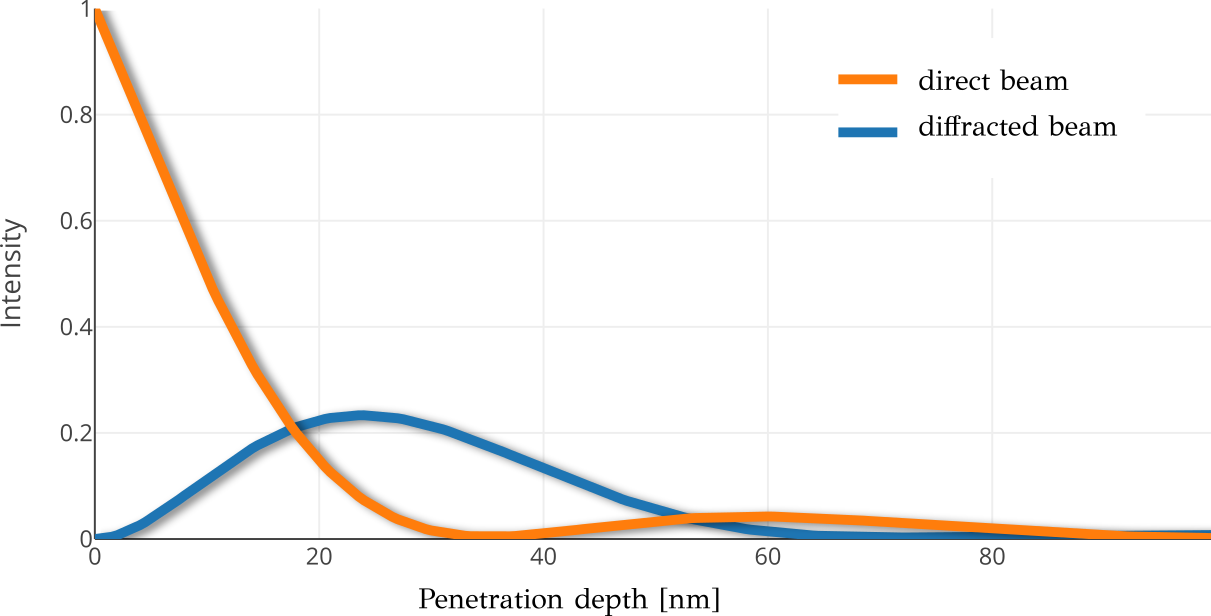
\includegraphics[width=0.84\linewidth]{Figures/fringes.png}
\caption[Thickness fringes.]{Penetration depth fringes for the direct and diffracted beams for a perfect centrosymmetric crystal.}
\label{Fig:fringes}

\end{figure}
%---------


Figure~\ref{Fig:fringes} shows exactly this periodic variation in the direct wave intensity  with penetration depth in crystal. In the TEM world this plot is known as thickness fringes, since if one would be to measure the transmitted intensity through a crystal shaped as a wedge and plot it as a function of sample thickness the same image would result. In the SEM case we can think of it as variation in the beams intensity as they travel inside the crystal. This plot can be achieved using any of the descriptions above. See \texttt{Task3.ipynb} for details.

A similarly oscillatory behaviour can be observed if we were to plot the intensity of the two beam as a function of deviation from the Bragg angle as we did in Fig.~\ref{Fig:rocking}. The name of rocking curves comes from the TEM world as well. Notice that the diffracted beam contributes only when very close to the Bragg angle. 


\begin{figure}[ht]
    \centering
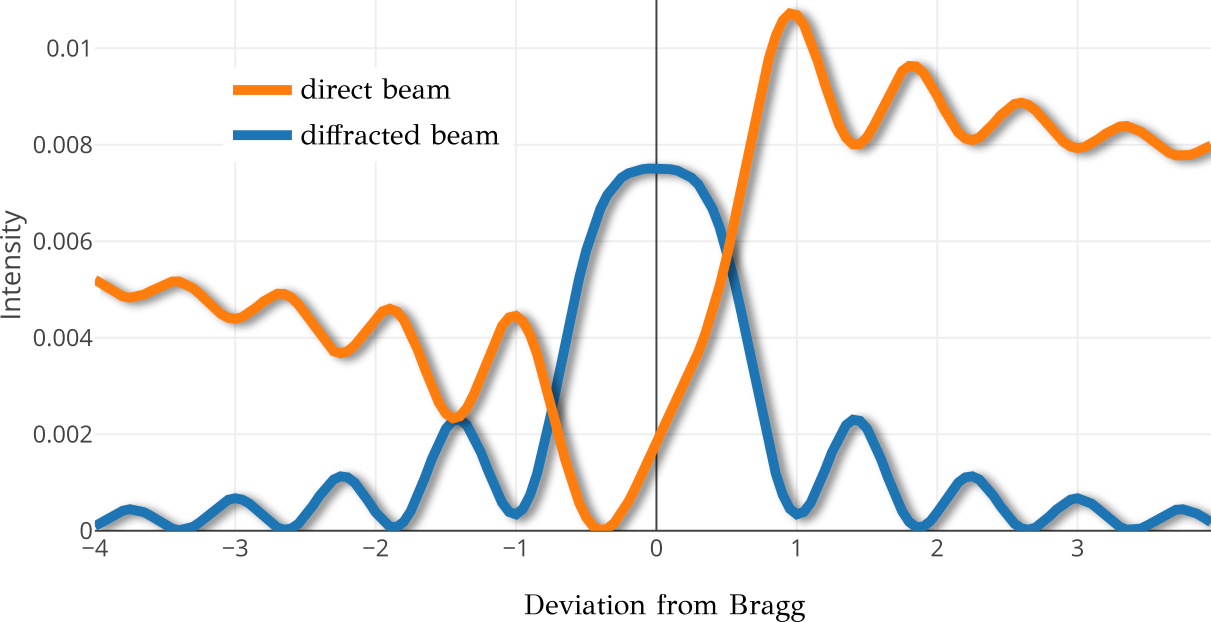
\includegraphics[width=0.84\linewidth]{Figures/rocking.png}
\caption[Rocking curves.]{Rocking curves for the direct and diffracted beams for a perfect centrosymmetric crystal. }
\label{Fig:rocking}

\end{figure}
%---------
